%% \documentclass{sig-alternate}
\documentclass[conference]{IEEEtran}

\usepackage{amssymb}
\usepackage{verbatim}
\usepackage{times}
\usepackage{graphicx}
\usepackage{epsfig}
\usepackage{url}
\usepackage{txfonts}
\usepackage{xspace}
\usepackage{float}
\usepackage{latexsym}
%\usepackage{natbib}
\usepackage{alltt}
\usepackage{color}
\usepackage{textcomp}
\usepackage{balance}
%\usepackage[pass,letterpaper]{geometry}
\usepackage[ruled,vlined]{algorithm2e}
\usepackage{enumitem}

\setlength{\paperheight}{11in}
\setlength{\paperwidth}{8.5in}
\usepackage[pass]{geometry}
\setlength{\textfloatsep}{0.4\baselineskip}

\begin{document}

\newcommand{\ie}{\textit{i.e.,} }
\newcommand{\eg}{\textit{e.g.,} }
\newcommand{\subject}[1]{\texttt{\small #1}}
\newcommand{\rules}{{\mathcal R}}
\newcommand{\tests}{{\mathcal T}}
\newcommand{\elemexists}{\mt{exists}}
\newcommand{\elemenabled}{\mt{enabled}}
\newcommand{\elemexplored}{\mt{explored}}
\newcommand{\note}[1]{{\color{red}$[$ \bf #1 $]$}}
\newcommand{\lang}[1]{\texttt{\scriptsize #1}}
\newcommand{\CodeIn[1]}{\small{\texttt #1}}
\newcommand{\tool}{\textsc{buster}}
\newcommand{\exhaust}{\textsc{exhaust}}
\newcommand{\choco}{\textsc{choco}}
\newcommand{\wateg}{\textsc{wateg}}

\title{Test Generation from Business Rules}

\author{
\IEEEauthorblockN{Simon Holm Jensen}
\IEEEauthorblockA{Snowflake Computing \\ simon@hjensen.net}
\and
\IEEEauthorblockN{Suresh Thummalapenta}
\IEEEauthorblockA{Microsoft Corporation \\ suthumma@microsoft.com}
\and
\IEEEauthorblockN{Saurabh Sinha}
\IEEEauthorblockA{IBM Research \\ saurabhsinha@in.ibm.com}
\and
\IEEEauthorblockN{Satish Chandra}
\IEEEauthorblockA{Samsung Research America \\ schandra@samsung.com}
}

%% \numberofauthors{4}
%% \author{
%% \alignauthor Simon Holm Jensen \\
%% \affaddr{Samsung Research America}\\
%% \email{s.jensen@samsung.com} 
%% \alignauthor Suresh Thummalapenta \\
%% \affaddr{Microsoft Corporation} \\
%% \email{suthumma@microsoft.com}
%% \alignauthor Saurabh Sinha \\
%% \affaddr{IBM Research India} \\
%% \email{saurabhsinha@in.ibm.com}
%% \and 
%% \alignauthor Satish Chandra \\
%% \affaddr{Samsung Research America} \\
%% \email{schandra@samsung.com}
%% }

\maketitle

\begin{abstract}
Enterprise applications are difficult to test because their intended
functionality is either not described precisely enough or described in
cumbersome business rules. It takes a lot of effort on the part of a test
architect to understand all the business rules and design tests that ``cover''
them, \ie exercise all their constituent scenarios. Part of the problem is that
it takes a complicated set up sequence to drive an application to a state in
which a business rule can even fire.  In this paper, we present a business rule
modeling language that can be used to capture functional specification of an
enterprise system. The language makes it possible to build tool support for rule
authoring, so that obvious deficiencies in rules can be detected
mechanically. Most importantly, we show how to mechanically generate test
sequences---\ie test steps and test data---needed to exercise these business
rules. To this end, we translate the rules into logical formulae and use
constraint solving to generate test sequences.  One of our contributions is to
overcome scalability issues in this process, and we do this by using a novel
algorithm for organizing search through the space of candidate sequences to
discover covering sequences.  Our results on three case studies show the promise
of our approach.
\end{abstract}

\section{Introduction}

A business rule articulates some aspect of the expected functional behavior (or
a \textit{requirement}) of an enterprise application. Here is a simple business
rule that determines how an invoice total is determined in a billing
application~\cite{jbilling}:
%
\begin{quote}
{\small
	
The \textit{Balance Type} of a customer affects how invoice total is computed;
it can be one of the following:

\textit{None}: The customer's account will not hold a balance; instead all
charges accrued in an order will be included in the next invoice;
	
\textit{Credit}: The customer's account may accrue charges up to the set credit
limit.  Charges will automatically be paid from the users credit pool until the
set limit is reached.  Users are responsible for paying their credit debt as
well as any overages.

}
\end{quote}	
%
We will examine this rule closely later; for now, suffice it to say that the
requirements of an enterprise system are typically captured by a large number
(often, hundreds) of business rules such as the one above.

It is reasonable to expect functional testing of an enterprise system to
\textit{cover} its business rules, which is to say testing would exercise all
distinct scenarios described in each business rule.  For example, in the
preceding rule, one of the scenarios to be covered is that a customer's balance
type is credit and the order amount exceeds the customer's credit limit.  A test
that covers this scenario would set up a customer with the~balance type as
\textit{credit} and a certain credit limit (say, \textit{100}), create an order
and add items to the order to bring the total to an amount (say, \textit{120})
that exceeds the credit limit for that customer, and finally create an invoice
for the order and verify the invoiced amount.
%Figure~\ref{fig:jbilling-flow} illustrates this flow.  
Although the values
\textit{credit}, \textit{100}, and \textit{120} can be identified from this
rule (by constraint solving), identifying a test sequence is also important to
apply those values at the right fields on the appropriate
screens in the application.
%\footnote{Not all fields on the screens in
%  Figure~\ref{fig:jbilling-flow} are constrained from the point of view of
%  exercising a particular scenario, but the application might still demand
%  sensible values for them. The tester is expected to make these up.}

%\begin{figure*}
%\centering
%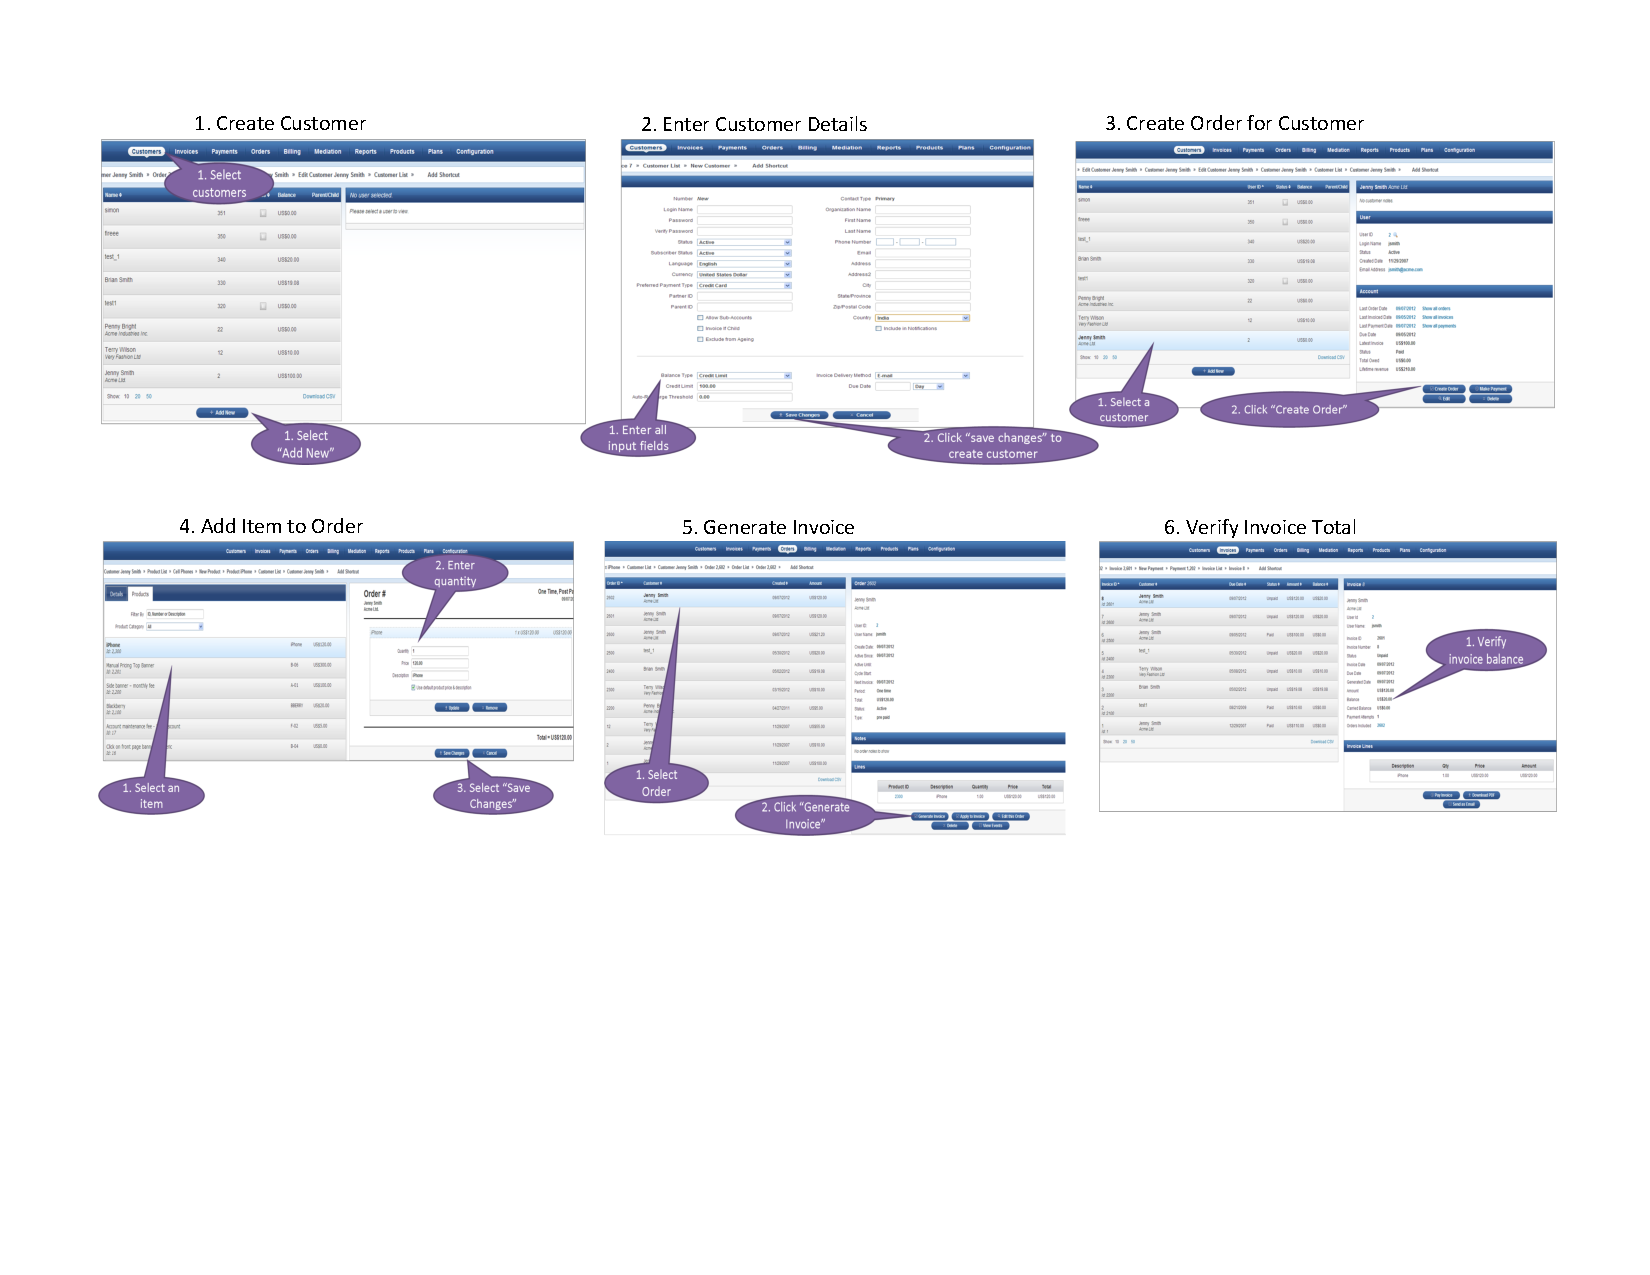
\includegraphics[trim=47 210 35 50,clip,width=\textwidth]{figs/jbilling-flow}
%\vspace*{-10pt}
%\caption{Test sequence for exercising a business rule from the
%  \subject{jBilling} application.}
%\vspace*{-7pt}
%\label{fig:jbilling-flow}
%\end{figure*}

It requires a carefully thought-out test scenario, \ie a sequence of test steps
as well as associated test data, \ie values to be entered in the relevant test
steps to exercise a business rule, or a scenario thereof.  Without systematic
test creation, testers may end up creating multiple tests that exercise the same
business rule, or a scenario thereof, over and over again without any additional
benefit (especially if they are incentivised by the number of tests created
rather than quality of the created tests), and more problematically, may neglect
to create tests for some other business rules.

In practice, due to time pressures, testers are more often ad-hoc than
methodical in creating test scenarios and test data.  One part of the problem is
that a realistic system can have hundreds of business rules written in plain
text, and it is difficult to get a global view of how the rules together
describe the application behavior.  A related part of the problem is that it may
need complex reasoning to piece together test sequences that cover each
scenario.  The net result is that, despite a lot of resources spent in testing,
bugs still escape into field.

\hyphenation{non-prog-ram-mers}

Our vision is to make testing of enterprise software more tool-based, by
adapting technology developed for automated and systematic test generation for
programs. In this vision, business rules would be written in a structured
notation that allows mechanized analysis.  Special editors could be created
to enable non-programm\-ers to capture business rules in a structured notation;
this is an independent challenge in \textit{end-user} programming.  A tool would
validate business rules and point out any ambiguities or omissions that it can
detect.  After the business rules pass validation, another tool would generate
test sequences and test data to exercise the application thoroughly as well as
without redundancies.

We have built a system to partially fulfil this vision.  In the rest of the
introduction, we give an overview of our system, describe some of the challenges
in automating test generation for covering business rules, and summarize our
results.

%Randomly generated test data cannot be expected to suffice for enterprise
%applications with complex rules. Also, systematic test-generation approaches
%based on program analysis (\eg \cite{Emmi:2007,Li:2010,Marcozzi:2012,Pan:2011})
%cannot be expected to tackle enterprise applications, which use a mix of
%multiple language and database technologies in their implementation. Moreover,
%these techniques are directed toward attaining simple forms of code coverage,
%such as statement or branch coverage, rather than coverage of complex business
%rules.

\subsection{An Overview}

Enterprise systems of interest to us are transaction-oriented, which means that
they consist of a set of transactions or operations (\eg create a customer, add
an item to an order, and so on) that operate on databases.  A business rule
applies to a particular operation supported by the system.  Formally, a business
rule describes the relation between the database state before and after the
operation.  Figure~\ref{fig:invoice} shows formalization of the business rule
quoted informally at the beginning of this section.  It says that the operation
refers to an invoice record, \subject{inv}, and modifies specific attributes of
\subject{inv}.  There are three scenarios that occur in this rule.  The first
scenario applies when the customer to which the invoice refers has balance type
\subject{None}; the \textit{precondition} is shown on the left of the first
arrow.  Note that the invoice has references to the customer to which this
invoice pertains and an order created in the system; in a relational database,
these would be foreign keys in the customer and order tables.  The second
scenario applies when the customer has balance type \subject{Credit} and the
credit limit is sufficient to cover the order total.  The third scenario applies
when the customer has balance type \subject{Credit}, but the order total exceeds
the credit limit.  In each scenario, the effect of the operation is to compute
invoice total and update the customer's residual credit limit; this effect, or
\textit{postcondition}, is shown to the right of the arrow.  Note that business
rules refer to the state observable at transaction boundaries; intermediate
program states encountered in the implementation while a transaction is in
process, are not important to business rules.

\begin{figure}
\centering
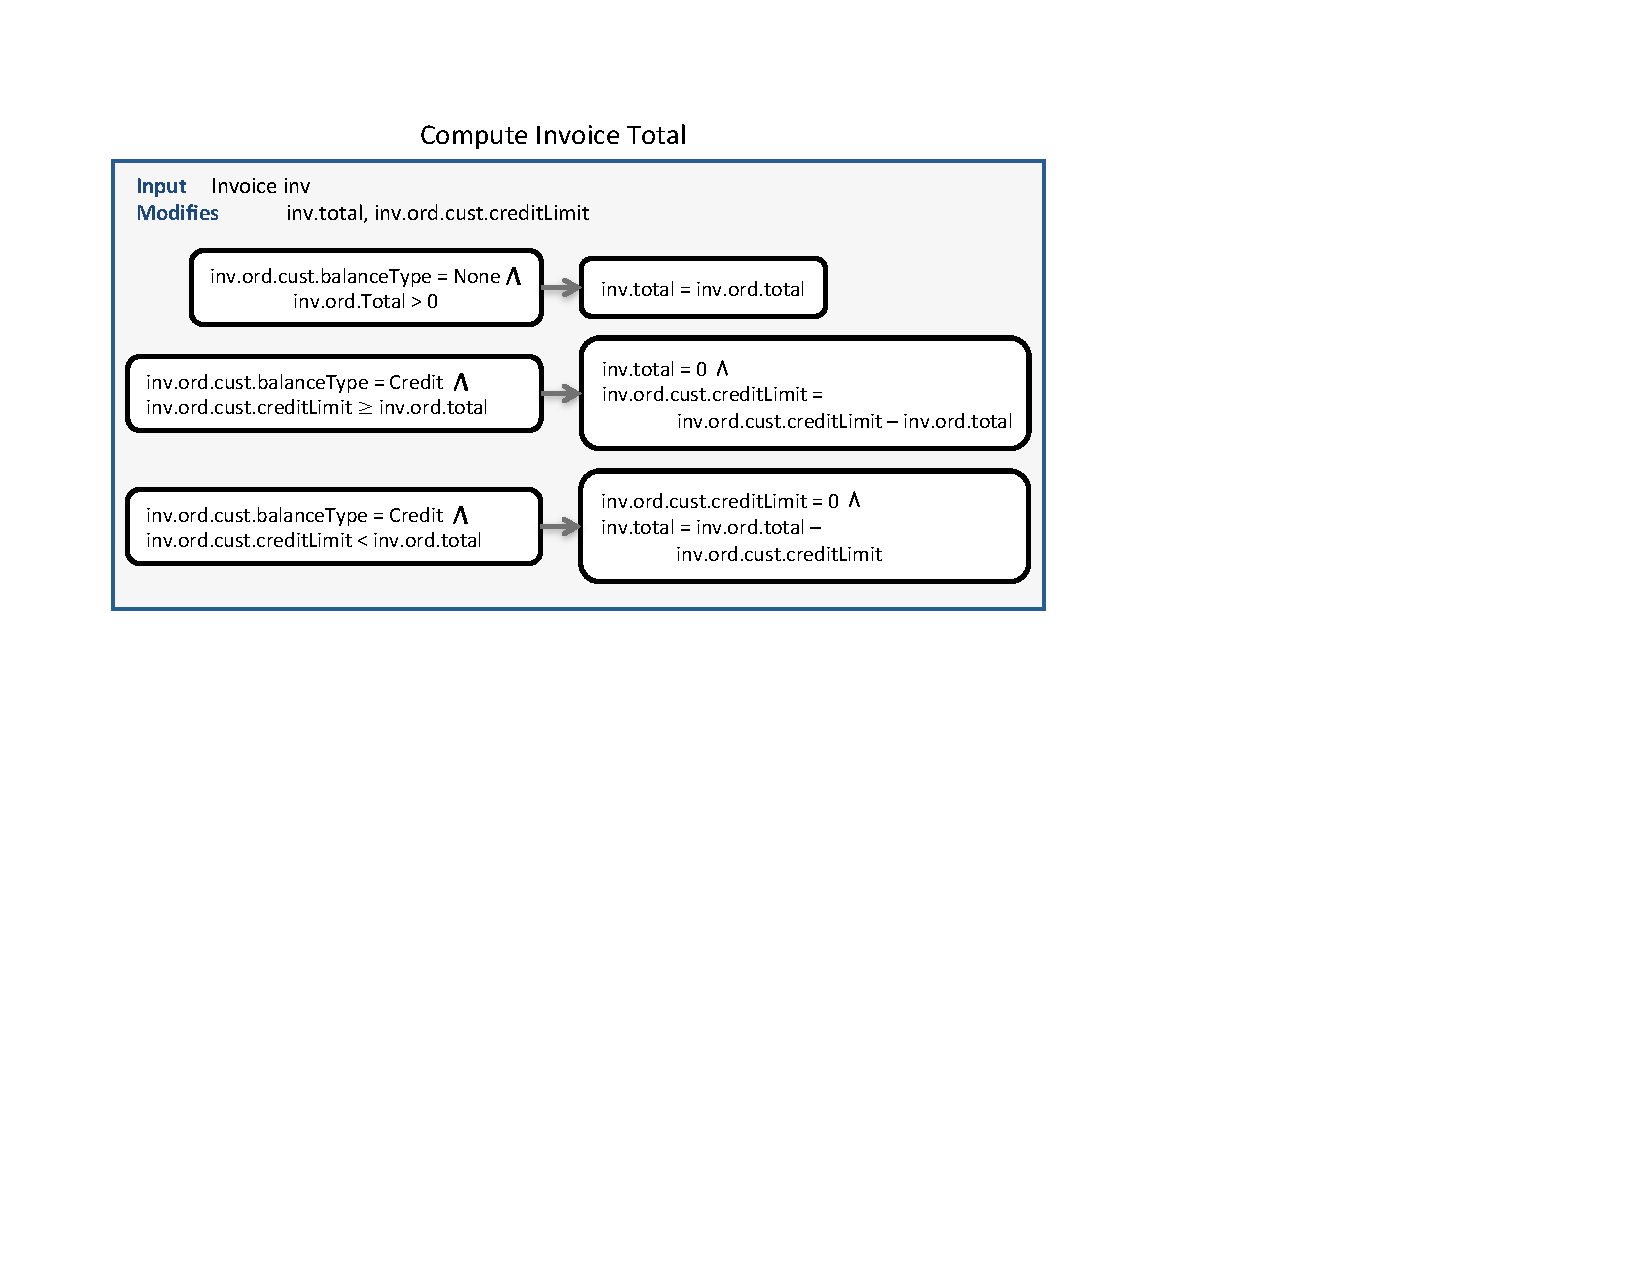
\includegraphics[trim=55 320 286 54,clip,width=\columnwidth]{figs/invoice}
\vspace*{-18pt}
\caption{Business rule for computing invoice amount.}
\label{fig:invoice}
\end{figure}

Covering a business rule means to exercise each of its constituent scenarios,
referred henceforth as \textit{rule parts}.  To cover the three rule parts shown
in Figure~\ref{fig:invoice}, it is necessary to create (separately) each of the
three preconditions and, in each case, verify that the postcondition holds after
the operation.  This brings us to the main difficulty in creating tests:
appropriate database state, such as a customer with a certain balance type and
an order with a certain amount, needs to be established before any of these
scenarios can be exercised.  In the \subject{jBilling} application's web
interface, it requires entering appropriate data step-wise in six distinct pages
to bring the application to a state at which these rule parts can be exercised.
%We showed in
%Figure~\ref{fig:jbilling-flow} the steps that would be required to create these
%preconditions.  
How can we identify these steps, and the data to~be entered in
each of the steps, automatically to cover a rule part?

Our observation is that the steps required to drive the database state to a
desired precondition are carried out by operations, and those operations too
would have rules that specify their functionality.  (In \subject{jbilling}, each
operation is triggered by entering appropriate data and clicking on ``submit''
on a web page specific to that operation.) We could then use business rules as
``state transformers'' and piece together a sequence of operations to arrive at
a desired state.  The advantage of looking at business rules as state
transformers is that we can adapt the technology developed for test generation
on \textit{programs} for the problem at hand.\footnote{We clarify, though, that
  business rules are themselves not executable programs; rather they only are an
  abstract description of the functionality of a program.}  The disadvantage of
relying on business rules to act as state transformers is that they need to be
specified to a certain level of detail for them to work out as state
transformers; this is generally not a big problem---practioners tend to write
business rules with an intention to be complete---but their intended use as
input to test generation process does increase expectations from the rules and,
therefore, from the analysts who write them.

\subsection{Our Approach and Results}

At a high level, the idea is to use backward analysis to piece together a
sequence of operations to arrive at a desired state.  We look for an operation
whose business rule has a rule part whose postcondition would imply the desired
precondition.  Such an operation, if executed in a way that the specific rule
part applies, would establish the desired state.  The operation may require some
user-provided values, but may partially rely on prior database state. The
process is repeated until no prior database state is assumed---that is, all the
database state is established by operations identified in the process.

Consider the second rule part shown in Figure~\ref{fig:invoice}. To satisfy the
precondition of the rule part, a customer with balance type \subject{Credit},
and an associated credit limit, needs to be created first. Then, an order whose
total does not exceed the customer's credit limit needs to be generated, which
involves adding items with suitable prices to the order. Only after this state
has been set up, the operation for invoice generation can be invoked. An
operation sequence and test data (we explain the notation in
Section~\ref{sec:approach}) that achieves this is:

\vspace*{-4pt}%
{\scriptsize
\begin{alltt}
 State st; BalanceType bt = Credit; int crLimit = 100, price = 20;
 Customer cust = CreateCustomer(st, bt);
 Customer cust1 = AddCreditLimit(cust, crLimit);
 Order ord = CreateOrder(cust1);
 Item item = CreateItem(int price);
 Order ord1 = AddItemToOrder(ord, item);
 Invoice inv = GenerateInvoice(ord1);  
\end{alltt}}%
\vspace*{-5pt}

The idea of backward traversal is definitely not novel; it is reminiscent of
weakest preconditions.  Our contribution is to make this idea work in the
context of business rules.  In general, the space of possible operation
sequences can be large, in which only a few sequences cover the target rule
part. Thus, the challenge is to search this space soundly, but efficiently in a
goal-driven manner. Specifically, our technique builds the sequence
incrementally using constraint solving. If the logical formula for a sequence is
not satisfiable, it extracts the unsatisfied core of the formula and constructs
new candidate sequences by considering only those operations and rule parts
whose postconditions are compatible with the unsatisfied core. In this way---and
using additional optimizations---the technique can prune out large parts of the
search space and efficiently narrow down to the covering sequences.

The sequencing of operations done by our algorithm is also reminiscent of AI
planning~\cite{Weld94} where actions with pre- and postconditions are sequenced
by a planner algorithm using forward or backward chaining. We discuss the
connection in the related work section; in brief, the algorithms for planning
would have to be fortified with the same kinds of optimizations as mentioned
above to be practical for our use.

An important ingredient of our approach is a notation for capturing business
rules formally, which enables mechanized analysis for test generation. Moreover,
prior to test generation, formally specified rules can be checked for
consistency and completeness properties.  The notation is designed to be natural
for use by architects, and while there is concern of a learning curve whenever a
notation has to be adopted, the industry has been moving toward
structured rule description languages (e.g. JBoss~\cite{JBoss},
ILOG~\cite{ILog}, and RuleML~\cite{RuleML}).  We believe the payoff by way of
consistency checks and automatic test coverage would further spur adoption of
structured rule languages.

We have implemented a prototype system, which includes a business rule editor
(an Eclipse plug-in) and automated analyses for rule checking and test
generation. Our preliminary results illustrate the promise of the approach: for
77~rule parts, modeled from three applications, our technique generated covering
sequences and test data for 99\% of the rule parts and missed only one rule part
(which could not be covered because of limitations of the underlying constraint
solver). By comparison, a technique that performs exhaustive (unguided) search
could cover 79\% of the rule parts, although it explored substantially more
candidate sequences than our technique.

%\paragraph*{Contributions}
The contributions of this paper are as follows:
\begin{itemize}[noitemsep]
\item We describe a notation for describing business rules formally, and articulate
  a set of well-formedness properties that can be checked mechanically. We have 
  also developed an Eclipse plugin for our rule language.
\item We describe an algorithm that can mechanically construct test sequences
  that cover the business rules of a model. The algorithm uses a
  novel optimization to prune the search space. We have implemented
  the algorithm. % in a tool called \tool{}.
\item To evaluate our approach, we have formalized the business rules
  of three enterprise systems and used \tool{} to generate test
  sequences. Using our approach we are able to generate tests for 99\%
  of the rule parts.
\end{itemize}

%In Section~\ref{sec:model}, we describe our notation for modeling business
%rules and present four well-formedness properties of
%models. In Section~\ref{sec:example}, we present the running example
%model, JBilling. In Section~\ref{sec:approach} we describe our approach including several
%optimizations. In Section~\ref{sec:eval} is the experimental evaluation using
%our implementation \tool{} and in Section~\ref{sec:related} we discuss related
%research.   


\newcommand{\term}{\textit}
\newcommand{\lit}{\texttt}

\section{Rule Modeling and Checking}
\label{sec:model}

In this section, we discuss the notation for modeling business rules and the
static checking performed on formally captured rules. Although there exist
business-rule management systems, such as JBoss~\cite{JBoss}, ILOG~\cite{ILog},
and RuleML~\cite{RuleML}, we found that they do not easily support automated
test generation for exercising transaction-oriented rules. As illustrated in the
Introduction, covering such rules can involve chaining a sequence of operations
to bring the system to a state in which a rule is applicable. For example,
coverage of the invoice computation rules (Figure~\ref{fig:invoice}) requires a
customer with a particular balance type and order amount; establishing this
state involves putting together an operation sequence along with suitable test
data. This suggests an ``operation centric''~modeling of rules. In the existing
rule-modeling notations, such as the ILOG and JBoss Drools rule languages, a
rule is essentially an if-then construct, where various conditions that control
actions can be expressed. Our notation models rules in the \textit{context of
  operations} and, thus, more naturally supports operation chaining for
automated test generation.

%% are not expressive enough to model complex transaction-oriented rules.
%% For example, in the ILOG and JBoss Drools rule language, a rule is essentially
%% an if-then condition, where various conditions that control actions can be
%% expressed.

\begin{figure}[t]
\centering
{\footnotesize
\tabcolsep=3pt
\begin{tabular}{lll}
\term{RuleSpec} & ::= & \term{Entities} \term{Operations} \term{Triggers} \\
\\
\term{Entities} & ::= & \term{Entity} \term{Entities} $|$ $\epsilon$ \\
\term{Entity} & ::= & \term{Enum} $|$ \term{Object} \\
\term{Enum} & ::= & \lit{enum} \term{ID} \{ \term{EnumVals} \} \\
\term{EnumVals} & ::= & \term{ID} \term{EnumVals} $|$ $\epsilon$ \\
\term{Object} & ::= & \lit{object} \term{ID} \{ \term{VarDecl} \} \\
\\
\term{Operations} & ::= & \term{Operation} \term{Operations} $|$ $\epsilon$ \\
\term{Operation} & ::= & \lit{operation} \term{ID} \{ \term{Input}
\term{Creates} \term{Modifies} \term{Rules} \term{Next} \} \\
\term{Input} & ::= & \lit{input} : \term{VarDecl} \\
\term{Creates} & ::= & \lit{creates} : \term{VarDecl} \\
\term{Modifies} & ::= & \lit{modifies} : \term{VarDecl} \\
\term{Rules} & ::= & \term{Rule} \term{Rules} $|$ $\epsilon$ \\
\term{Rule} & ::= & \lit{group} \term{ID} \{ \term{RuleParts} \} \\
\term{RuleParts} & ::= & \term{RulePart} \term{RuleParts} $|$ $\epsilon$ \\
\term{RulePart} & ::= & \lit{rule} \term{ID} \{ \lit{pre} : \term{Expr} ;
\lit{post} : \term{Expr} \} \\
\term{Next} & ::= & \lit{next} : \term{ID} $|$ $\epsilon$ \\
\\
%\term{Triggers} & ::= & \term{ID} $\rightarrow$ \term{ID} \term{Triggers} | $\epsilon$ \\
%\\
\term{VarDecl} & ::= & \term{TypeName} : \term{ID} \term{VarDecl} | $\epsilon$
\\
\term{TypeName} & ::= & \lit{bool} $|$ \lit{int} $|$ \lit{float} $|$ \lit{string} $|$
\lit{set<\term{\textrm{TypeName}}>} $|$ \term{ID} \\
\term{Expr} & ::= & $\ldots$ \\
\end{tabular}
}
\vspace*{-3pt}
\caption{Partial rule-modeling syntax.}
\vspace*{0pt}
\label{fig:model-syntax}
\end{figure}

\subsection{Rule-Modeling Language}

%% We model rules in the context of operations in the system under test.
An operation is described by a set of input entities, a set of created entities,
a set of modified entities, and a set of rules, where each rule consists of a
set of precondition-postcondition pairs. For example, Figure~\ref{fig:invoice}
shows the operation for computing invoice totals in \subject{jBilling}. The
rules associated with this operation, which govern how the invoice total and the
customer's credit limit are updated, are modeled with the operation in the form
of precondition-postcondition pairs.

Figure~\ref{fig:model-syntax} presents the syntax of the rule-modeling language
(for clarity, we omit some of the details and present only the important parts
of the language). A \textit{rule specification} consists of entities and
operations. An \textit{entity} can be an object (\eg invoice, order, customer)
or an enumerated type (\eg a customer's balance type can be \subject{None},
\subject{Credit}, or \subject{Prepaid}).
%% The key part of the syntax, which models rules, is based on
%% operations.
Formally, an \textit{operation} ${\cal O}$ is the tuple $(I, C, M, R, o_n)$,
where $I$ is the set of input entities read during the execution of ${\cal O}$,
$C$ is the set of entities created by ${\cal O}$, $M$ is the set of entities
whose attributes are modified by ${\cal O}$, $R$ is the set of rules that
describe the behavior of ${\cal O}$, and $o_n$ is a succeeding operation that,
if specified, is the only operation that can execute after ${\cal O}$.

The notion of \textit{succeeding operation} can simplify the modeling of
coarse-grained operations that have many rules associated with them. Such an
operation can be broken down into a sequence of finer-grained operations---with
the sequence specified via the \subject{next} clause---that have simpler
rules. This lets the test-generation algorithm ensure that the atomic nature of
the coarse-grained operation is preserved in the finer-grained sequence: while
chaining operations, the algorithm avoids interleaving other operations in the
middle of a finer-grained operation sequence.  Moreover, such decomposition is
necessary when the rules of an operation have data dependences, which define an
implicit ordering among the rules. %% One of the well-formedness
%% properties that we impose on rule specifications (discussed in
%% Section~\ref{sec:checking}) is data independence among the rules of an
%% operation.

A \textit{rule} $R = \{r_1, r_2, \ldots, r_k\}, k \geq 1,$ consists of a set of
rule parts. A \textit{rule part} $r$ is a precondition-postcondition pair, $p
\Longrightarrow q$, where $p$ and $q$ are boolean formulas such that if $p$
holds in the state before the operation, $q$ is true in the state resulting from
the execution of the operation.
%% If the precondition of a rule part is true, we say that the rule is
%% \textit{applicable}.
The rule shown in Figure~\ref{fig:invoice} has three rule parts, each of which
consists of a precondition and a postcondition.

%% The first rule part pertains to the case where the customer's balance type is
%% \subject{None}; the second rule part is for the case where the balance type is
%% \subject{Credit} and the credit limit exceeds or equals the order total; the
%% third rule part covers the case where the balance type is \subject{Credit} and
%% the order total exceeds the credit limit.

%Often in enterprise systems, the execution of an operation or a transaction
%automatically triggers other transactions or operations. For example, in
%\subject{jBilling}, customers with balance type \subject{Prepaid} have the
%option of getting their prepaid limit automatically recharged if it falls below
%a threshold amount. Our rule-modeling syntax accommodates this via the
%\subject{Triggers} clause, using which the triggers relation between a pair of
%operations---where the first operation automatically triggers the second
%operation---can be specified.

%% The primitive types include boolean, integer, float, and string. The model also
%% accommodates sets of these types.\footnote{In the currently implemented system,
%%   set types are handled in a restricted manner: by limiting the set size to two
%%   and specifying the predicates over a set in terms of its (two) elements.}

\subsection{Rule Checking}
\label{sec:checking}
 
We define a few well-formedness properties on rule specifications to ensure
consistency and completeness, and that also facilitate operation chaining for
test generation. These properties are amenable to mechanical checking. Thus, we
envision that the rules can be iteratively refined in a rule editor, based on
automatic semantic checking for property violations. %%  (in addition to syntactic
%% checking for conformance to the modeling syntax).

\paragraph*{Property 1: Rule-part Disjointedness}
In our notation, a rule part is intended to represent disjoint preconditions so
that when a rule is applicable, the precondition of only one rule part is true;
consequently, there is no ambiguity in identifying the relevant rule part for an
applicable rule. Formally, we define this property as follows. Let $R= \{r_1,
r_2, \ldots, r_k\}$ be a rule such that $k \geq 2$. Then, for all $r_i, r_j \in
R$ where $ r_i \coloneqq (p_i \Longrightarrow q_i)$ and $r_j \coloneqq (p_j
\Longrightarrow q_j)$, $(p_i \wedge p_j)$ must not be satisfiable. A simple
example of a rule specification that violates this property is $p_i = (a > 0)$
and $p_j = (a < 10)$; this specification represents ambiguous behavior when, for
example, $a = 5$.  The rule parts illustrated in Figure~\ref{fig:invoice} have
disjoint preconditions.

To check that a rule satisfies this property, we enumerate all pairs of rule
parts and, for each pair (with preconditions $p_i$ and $p_j$), determine whether
the boolean formula $(p_i \wedge p_j)$ has a solution; if it does, we flag a
violation of the property.

\paragraph*{Property 2: Rule-part Completeness}
This property is intended to ensure that a rule specifies the complete operation
behavior for the variables mentioned in the rule. Let $R= \{r_1, r_2, \ldots,
r_k\}$ be a rule such that $k \geq 2$ and $r_i \coloneqq (p_i \Longrightarrow
q_i)$. Then, $\neg(p_1 \vee p_2 \vee \ldots \vee p_k)$ must not be
satisfiable. For example, the rule consisting of two rule parts with
preconditions $(a < 5)$ and $(a > 10)$, respectively, violates the completeness
property because the operation behavior for $5 \leq a \leq 10$ is left
unspecified.  To verify this property, our technique checks, for each rule that
has two or more parts, whether the formula $\neg(p_1 \vee p_2 \vee \ldots \vee
p_k)$ has a solution.

%\paragraph*{Property 3: Rule Compatibility}
%The rule compatibility property requires that for any set of applicable rules of
%an operation, the postconditions of their relevant rule parts must not be
%conflicting. To illustrate, consider rules $R_1 = \{r_1\}$ and $R_2 = \{r_2\}$
%for an operation, such that $r_1 \coloneqq ((a > 0) \Longrightarrow (total =
%10))$, $r_2 \coloneqq ((b > 0) \Longrightarrow (total = 20))$, and the two
%preconditions are not disjoint (\ie $(a > 0) \wedge (b > 0)$ is
%satisfiable). This pair of rules violates the compatibility property because the
%postconditions are conflicting, whereas the corresponding preconditions can be
%true simultaneously---the first precondition does not constrain the value of
%\subject{b}, and the second precondition does not constrain the value of
%\subject{a}. Thus, when both preconditions are true, it is not clear what value
%\subject{total} would have after the operation.
%
%To state this property formally, let $r_1 \coloneqq (p_1 \Longrightarrow q_1)$
%and $r_2 \coloneqq (p_2 \Longrightarrow q_2)$ be the relevant rule parts of two
%applicable rules of an operation. Then, if $(p_1 \wedge p_2)$ is satisfiable,
%$(q_1 \wedge q_2)$ must be satisfiable. To verify this, our technique enumerates
%all pairs of rules for an operation. Then, for each pair $R_1$ and $R_2$, the
%techniques lists each combination $(p_1, p_2)$ of the preconditions of $R_1$ and
%$R_2$, and checks the satisfiability of $(p_1 \wedge p_2)$ and the conjunction
%of the corresponding postconditions.
%
%If two rules violate the compatibility property, it might in fact indicate that
%their rule parts can be merged into one rule. In the preceding example, $R_1$
%and $R_2$ could be merged into one rule with two rule parts $R_m = \{r_{m_1},
%r_{m_2}\}$, where $r_{m_1} \coloneqq (a > 0) \Longrightarrow (total = 10)$ and
%$r_{m_2} \coloneqq (a \leq 0 \wedge b > 0) \Longrightarrow (total = 20)$. Note
%adding the conjunct $a \leq 0$ (the negation of the precondition of $r_1$) to
%the precondition of $r_{m_2}$ makes the two preconditions disjoint, which
%ensures that $R_m$ satisfies the rule-part disjointedness
%property. Alternatively, the negation of the precondition of $r_2$ could be
%added to the precondition of $r_{m_1}$ to satisfy this property.

\paragraph*{Property 3: Rule Independence}
Finally, we enforce the restriction that there can be no data dependence between
the postcondition of one rule and the precondition of another rule of the same
operation. This property ensures that there is no implicit ordering among the
rules of an operation. When such an ordering exists between two rules of an
operation, the operation should be split using the \subject{next} clause.

We formalize this property as follows. Let ${\cal R} = \{R_1, R_2, \ldots,
R_n\}$ be the rules associated with an operation. For any $R_i, R_j \in {\cal
  R}$, let $V_{i, \mathit{post}}$ be the set of variables used in the
postconditions of the rule parts of $R_i$ and $V_{j, \mathit{pre}}$ be the set
of variables used in the preconditions of the rule parts of $R_j$. Then, $V_{i,
  \mathit{post}} \cap V_{j, \mathit{pre}} = \emptyset$. The checking of this
property is straight forward: for each pair of rules for an operation, the
technique computes the sets of variables used in the preconditions of one rule
and the postconditions of the other rule, and verifies that the two sets are
non-intersecting. In future work, we plan to integrate more properties such
as safety and confluence properties~\cite{DBLP:conf/icst/BerstelL10}. 

\subsection{Guided Model Creation}

\begin{figure}[t]
\centering
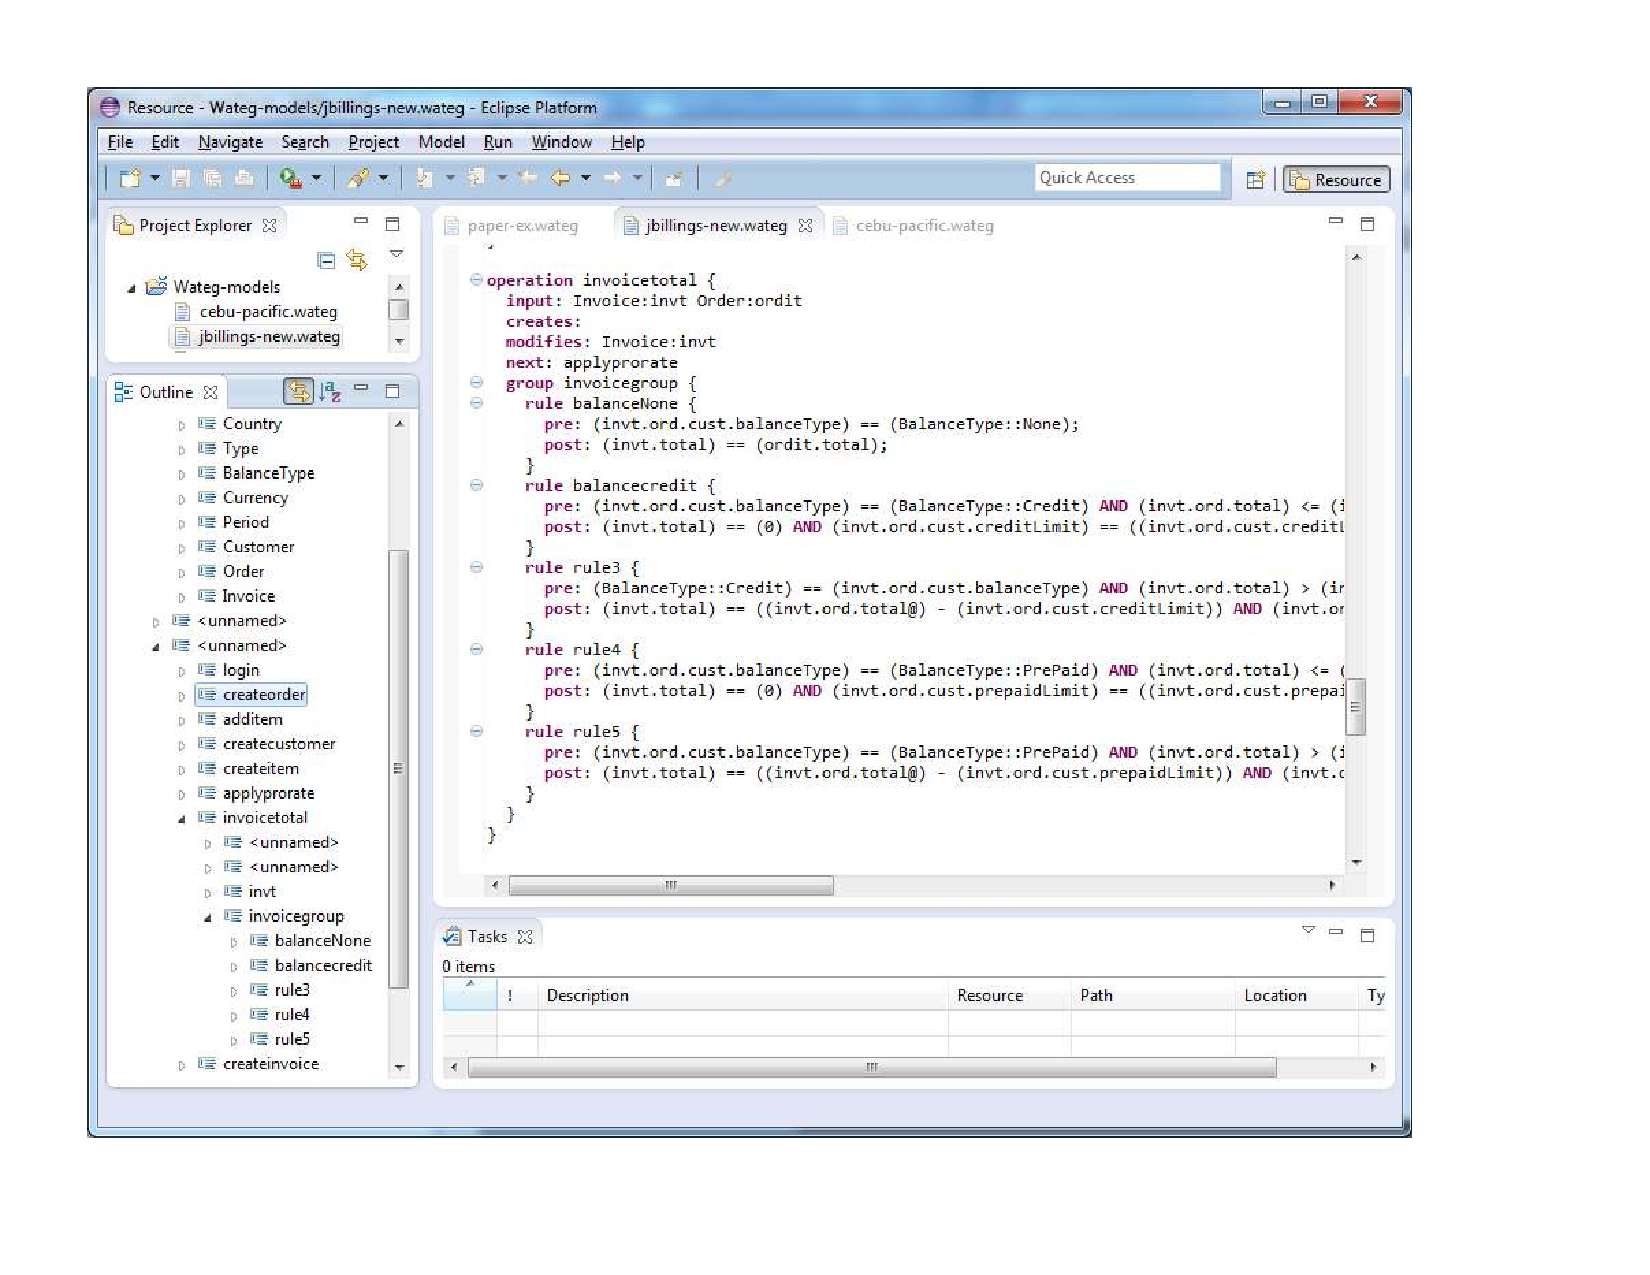
\includegraphics[trim=43 65 114 36,clip,width=\columnwidth]{figs/rule-editor.pdf}
\vspace*{-13pt}
\caption{Screenshot of the Eclipse-based rule editor.}
\vspace*{-0pt}
\label{fig:rule-editor}
\end{figure}

%% Our end goal of test generation requires accurate rule models. Moreover, we want
The modeling process must be realistic in that users should be able to create
and refine models in a tool-assisted manner, with immediate checking of, and
feedback on, errors in the models.  We have implemented such a rule editor as an
Eclipse plugin; Figure~\ref{fig:rule-editor} shows a screenshot of the
editor. The editor is built using Eclipse Xtext~\cite{xtext}, which is a general
framework for developing domain-specific and programming languages. Much like
any modern syntax-directed editor for a programming language, the rule editor
provides syntax highlighting, navigation features, auto completion, and
on-the-fly detection of syntax errors.  The user can also run a semantic checker
to detect violations of the well-formedness properties discussed
previously. Thus, the editor provides a convenient environment for writing
rules, in which the user is guided by automated checking and feedback.


\begin{table*}[t]
\caption{Formal specification of sample business rules in \subject{jBilling}.}
\centering
\tabcolsep=4pt
{\scriptsize
\begin{tabular}{|l|l|l|l|l|l|}
\hline
& & & & \multicolumn{2}{|c|}{Rules $(R)$} \\
\cline{5-6}
\multicolumn{1}{|c|}{Operation} &
\multicolumn{1}{|c|}{Inputs $(I)$} &
\multicolumn{1}{|c|}{Creates $(C)$} &
\multicolumn{1}{|c|}{Modifies $(M)$} &
\multicolumn{1}{|c|}{Description} &
\multicolumn{1}{|c|}{Formal Representation} \\
\hline \hline
Create & \{{\tt State,} & \{{\tt Customer}\} &
\multicolumn{1}{|c|}{$\emptyset$} &
$R_1$: The \textit{credit limit (crLimit)} of newly  &
$r_{1.1}$: $({\tt true}) \Longrightarrow ({\tt cust.state} = {\tt state} \; \wedge$ \\
Customer & {\tt BalanceType}\} & & & created customers should be \textit{zero} &
\hspace*{10pt}$ {\tt cust.balType} = {\tt  balType} \; \wedge {\tt cust.crLimit} = 0)$ \\
\hline
Create & \{{\tt Int}\} & \{{\tt Item}\} & \multicolumn{1}{|c|}{$\emptyset$} &
$R_2$: The price of an item must be greater &
$r_{2.1}$: $({\tt price} > 0) \Longrightarrow ({\tt item.price} = {\tt price})$ \\
Item & & & & than zero & \\
\hline
Create & \{{\tt Customer}\} & \{{\tt Order}\} &
\multicolumn{1}{|c|}{$\emptyset$} &
$R_3$: The \textit{total} of a newly created order &
$r_{3.1}$: $({\tt true}) \Longrightarrow$ $({\tt ord.total} = 0 \wedge {\tt ord.cust} = {\tt cust})$ \\
Order & & & & should be zero & \\
%% \cline{5-6}
%% & & & & Orders created in the month of &
%% $({\tt month} = {\tt Nov}) \Longrightarrow ({\tt ord.extraDiscount} = 1)$ \\
%% & & & & are eligible for a Thanksgiving &
%% $({\tt month} \neq {\tt Nov}) \Longrightarrow ({\tt ord.extraDiscount}
%% = 0)$  \\
%% & & & & discount of 5\% & \\
\hline
Generate & \{{\tt Order}\} & \{{\tt Invoice}\} &
\multicolumn{1}{|c|}{$\emptyset$} &
$R_4$: A customer's balance type determines &
$r_{4.1}$: $({\tt ord.total} > 0 \wedge {\tt ord.cust.balType} = {\tt None}) \Longrightarrow$ \\
Invoice & & & & how the invoice total is computed &
\hspace*{10pt}$({\tt inv.total} = {\tt ord.total})$ \\
& & & & (see complete rule in the Introduction) &
$r_{4.2}$: $({\tt ord.total} > 0 \wedge {\tt ord.cust.balType} = {\tt Credit} \; \wedge$ \\
& & & & &
\hspace*{10pt}${\tt ord.cust.crLimit} \geq {\tt ord.total}) \Longrightarrow$ \\
& & & & &
\hspace*{10pt}$({\tt inv.total} = 0 \; \wedge$ \\
& & & & &
\hspace*{10pt}${\tt ord.cust.crLimit} = {\tt ord.cust.crLimit@} - {\tt ord.total})$ \\
& & & & &
$r_{4.3}$: $({\tt ord.total} > 0 \wedge {\tt ord.cust.balType} = {\tt Credit} \; \wedge$ \\
& & & & &
\hspace*{10pt}${\tt ord.cust.creditLimit} < {\tt ord.total}) \Longrightarrow$ \\
& & & & &
\hspace*{10pt}$({\tt inv.total} = {\tt ord.total} - {\tt ord.cust.crLimit} \; \wedge$ \\
& & & & &
\hspace*{10pt}${\tt ord.cust.crLimit} = 0)$ \\
\cline{5-6}
& & & & $R_5$: If the customer's residence is in &
$r_{5.1}$: $({\tt ord.total} > 0 \wedge {\tt ord.cust.state} = {\tt NY})
\Longrightarrow$ \\ 
& & & & NY \textit{state}, an additional 2\% discount &
\hspace*{10pt}$({\tt inv.total} = {\tt ord.total} * (98 / 100))$ \\ 
& & & & is given while generating invoices &
$r_{5.2}$: $({\tt ord.total} > 0 \wedge {\tt ord.cust.state} = {\tt Other})
\Longrightarrow$ \\
& & & & &
\hspace*{10pt}$({\tt inv.total} = {\tt ord.total})$ \\
\hline
Add Credit & \{{\tt Customer,} & \multicolumn{1}{|c|}{$\emptyset$} &
\{{\tt Customer}\} &
$R_6$: The credit limit can be incremented for &
$r_{6.1}$: $({\tt cust.balType} = {\tt Credit} \wedge {\tt amount} > 0) \Longrightarrow$ \\
Limit & {\tt Int}\} & & & customers with balance type \textit{Credit} &
\hspace*{10pt}$({\tt cust.crLimit} = {\tt cust.crLimit@} + {\tt amount})$\\
\hline
%% Deactivate & \{{\tt Customer}\} & \multicolumn{1}{|c|}{$\emptyset$} &
%% \{{\tt Customer}\} &
%% Active customers can be deactivated &
%% $({\tt cust.status} = {\tt Active}) \Longrightarrow ({\tt cust.status} = {\tt Inactive})$ \\
%% Customer & & & & & \\
%% \hline
Add Item & \{{\tt Order}, {\tt Item}\} &
\multicolumn{1}{|c|}{$\emptyset$} & \{{\tt Order}\} &
$R_7$: Adding an item to an order increases &
$r_{7.1}$: $({\tt true}) \Longrightarrow ({\tt ord.total} = {\tt ord.total@} +
{\tt item.price})$ \\
to Order & & & & the order's total by the item's price & \\
\hline
\end{tabular}
}
\label{tab:bookstore-rules-spec}
\end{table*}

\section{Example Application Model}
\label{sec:example}

Before presenting our technique, we elaborate upon the billing application
example (\subject{jBilling}) mentioned in the previous sections: we explain
various operations and rules for the application, which we use subsequently to
illustrate our technique. To facilitate the illustration, we use a simplified
version inspired by the actual application.\footnote{\scriptsize
  \url{http://www.jbilling.com/}} (In the empirical evaluation, we modeled a
larger part of the application.) The model for \subject{jBilling} includes four
entities: \subject{Customer}, \subject{Item}, \subject{Order}, and
\subject{Invoice}.  Figure~\ref{fig:sample-app} shows the flow among some of the
operations, which create, read, or modify these entities. For example, operation
\subject{CreateCustomer} creates an instance of \subject{Customer}, whereas the
operation \subject{AddItemToOrder} modifies an \subject{Order} instance by
adding a new item to the order.

Table~\ref{tab:bookstore-rules-spec} presents the formal specification of the
\subject{jBilling} operations and rules. Columns~2--4 list, respectively, the
entities read, created, and modified by an operation. Columns~5 and 6 provide
informal descriptions and formal representations of the rules associated with an
operation.  \subject{GenerateInvoice} has two rules associated with it, whereas
all the other operations have only one rule associated with them. The first rule
for \subject{GenerateInvoice} has three rule parts, which determine how the
invoice total and the customer's credit limit are updated by the operation,
based on the customer's balance type.  The second rule for
\subject{GenerateInvoice} has two rule parts---which also determine the
computation of invoice total, this time based on the customer's state of
residence.

\begin{figure}[t]
\centering
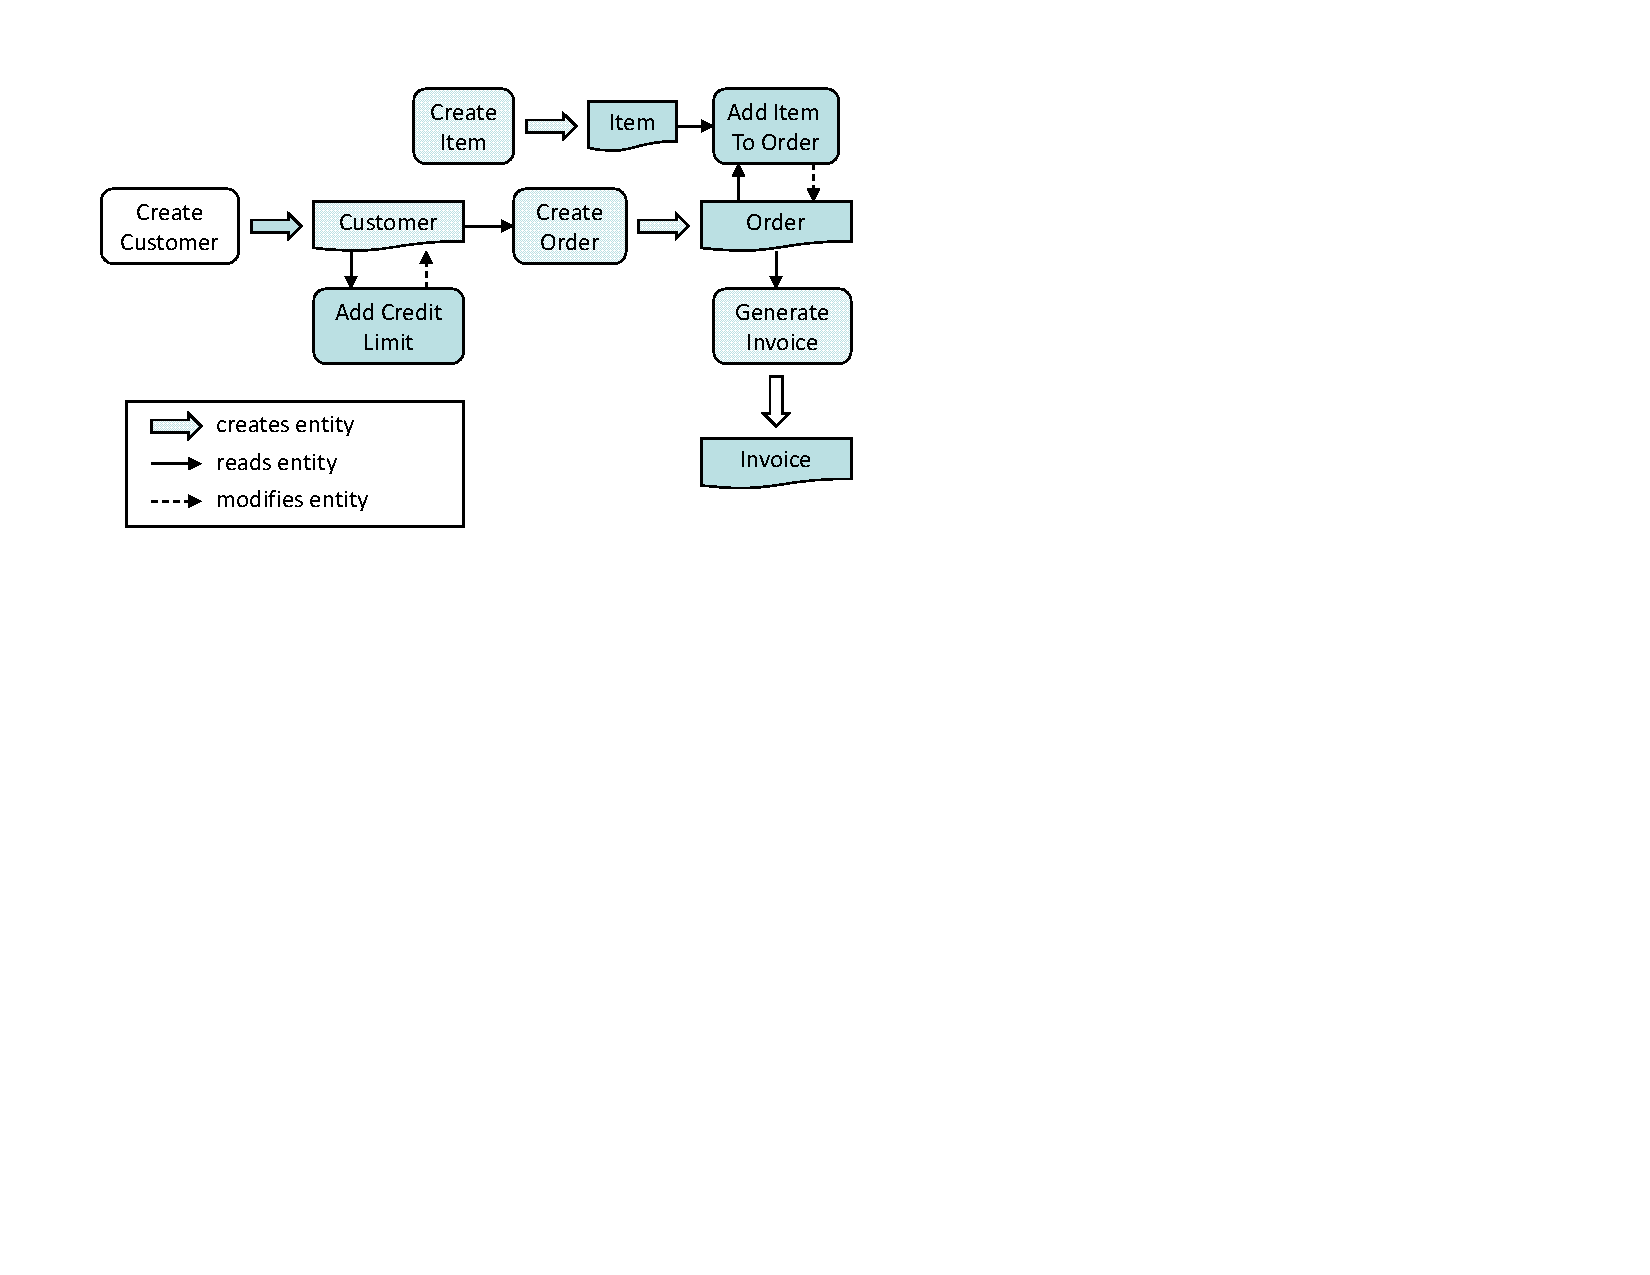
\includegraphics[trim=47 350 380 42,clip,width=.9\columnwidth]{figs/appModel.pdf}
\vspace*{-12pt}
\caption{Sample operations and their interactions in \subject{jBilling}.}
\vspace*{-0pt}
\label{fig:sample-app}
\end{figure}

The boolean expressions in the rule parts refer to the input/crea\-ted/modified
entities by names: \eg the rule part for \subject{CreateOrder} refers to the
input \subject{Customer} instance as \subject{cust} and the created
\subject{Order} instance as \subject{ord}. The expressions also refer to
attributes of the entities. For example, some of the relevant attributes of
\subject{Customer} are:

\vspace*{-5pt}
{\scriptsize
\begin{verbatim}
  Customer {
      State: state
      BalanceType: balType
      int: crLimit
  }
\end{verbatim}
}
\vspace*{-7pt}

where \subject{State} and \subject{BalanceType} are
enumerated types (\eg attribute \subject{BalanceType} can take two values---\subject{None}
or \subject{Credit}) and the attribute \subject{crLimit} is an integer.

If an expression needs to refer to the old and new values of an attribute (\ie
the values prior and subsequent to an operation invocation), the old value is
distinguished by appending `@' to the attribute name. For instance, consider the
postcondition in the rule for \subject{AddCreditLimit}: {\small ${\tt
    cust.crLimit} = {\tt cust.crLimit@} + {\tt amount}$}; this states that the
input credit amount is added to the customer's old credit limit to obtain the
new credit limit.

\section{Test generation}
\label{sec:approach}

Given an operation ${\cal O}$ and a target rule part $r$ in ${\cal O}$, our
technique attempts to generate a \textit{test sequence}, consisting of an
operation sequence and test data, that \textit{covers} $r$---that is, the
sequence produces all input entities of ${\cal O}$ in appropriate object states
to ensure that the precondition of $r$ is satisfied. The challenge is to search
for a covering sequence efficiently from a large set of candidate sequences. For
example, one of our experimental subjects, \subject{Cebu-pacific}, has eight
operations that accept an entity \subject{Ticket} as input and modify
it. Therefore, any sequence composed using one or more of these operations can
be a candidate sequence; however, different sequences and orderings produce
different object states of \subject{Ticket}. Our technique addresses this
challenge by exploring the large search space efficiently, in a goal-directed
manner, by ignoring sequences that are not likely to cover the target rule.

%% In general, it is often challenging to identify a test sequence that covers $r$,
%% since there can be a large number of candidate sequences and only a few
%% sequences produce desired object states that help cover $r$. For example, in one
%% of our subjects \subject{Cebu-pacific}, there are eight operations that accept
%% an entity \subject{Ticket} as input and modify that entity. Therefore, any
%% sequence composed using one or more of these operations is a valid sequence,
%% however, different sequences and also different orderings of those sequences
%% produce different object states of the \subject{Ticket} entity.  Our technique
%% addresses this challenge by efficiently exploring the large search space via
%% composing sequences incrementally.

%% Overall, our technique first enumerates sequences of operations (along with
%% selected rule parts in those operations) that create all input entities of
%% ${\cal O}$.  Next, for each sequence, it checks whether the sequence generates
%% the desired object states (for all input entities of ${\cal O}$) so that $r$ is
%% covered. If the sequence is satisfiable, our technique infers test data for all
%% inputs that are of primitive and enumerated types.  Otherwise, it identifies an
%% entity $e$ and its attribute $attr$ that needs to be modified to achieve the
%% desired object state. Next, it identifies candidate operations that modify
%% $attr$, composes new sequences using those candidate operations, and further
%% checks whether those new sequences are satisfiable. Our technique repeats this
%% process until it identifies a satisfiable sequence or reaches a user-defined
%% threshold of the maximum number of sequences to be explored.

\subsection{Terminology}

Before presenting the test-generation algorithm, we introduce some terminology
and definitions: we discuss two types of graphs (the dependence graph and the
operation flow graph) and define abstract and concrete operation sequences.

\subsubsection{Graphs}

\vskip -10pt
\paragraph*{Dependence Graph} A \textit{dependence graph} is a directed graph
that captures interactions of operations with entities: nodes in the graph
represent operations and entities, whereas edge represent creates, reads, and
modifies relations.  A \textit{creates edge} or a \textit{modifies edge} from an
operation to an entity indicates that the operation creates or modifies that
entity; a \textit{reads edge} from an entity to an operation indicates that the
operation reads the entity.  Figure~\ref{fig:sample-app} shows the dependence
graph for our example application.

%% While composing sequences, our technique uses this graph to ensure that the
%% dependencies among operations are satisfied.  Figure~\ref{fig:sample-app}
%% shows the dependency graph for our example application.

\begin{figure}[t]
\centering
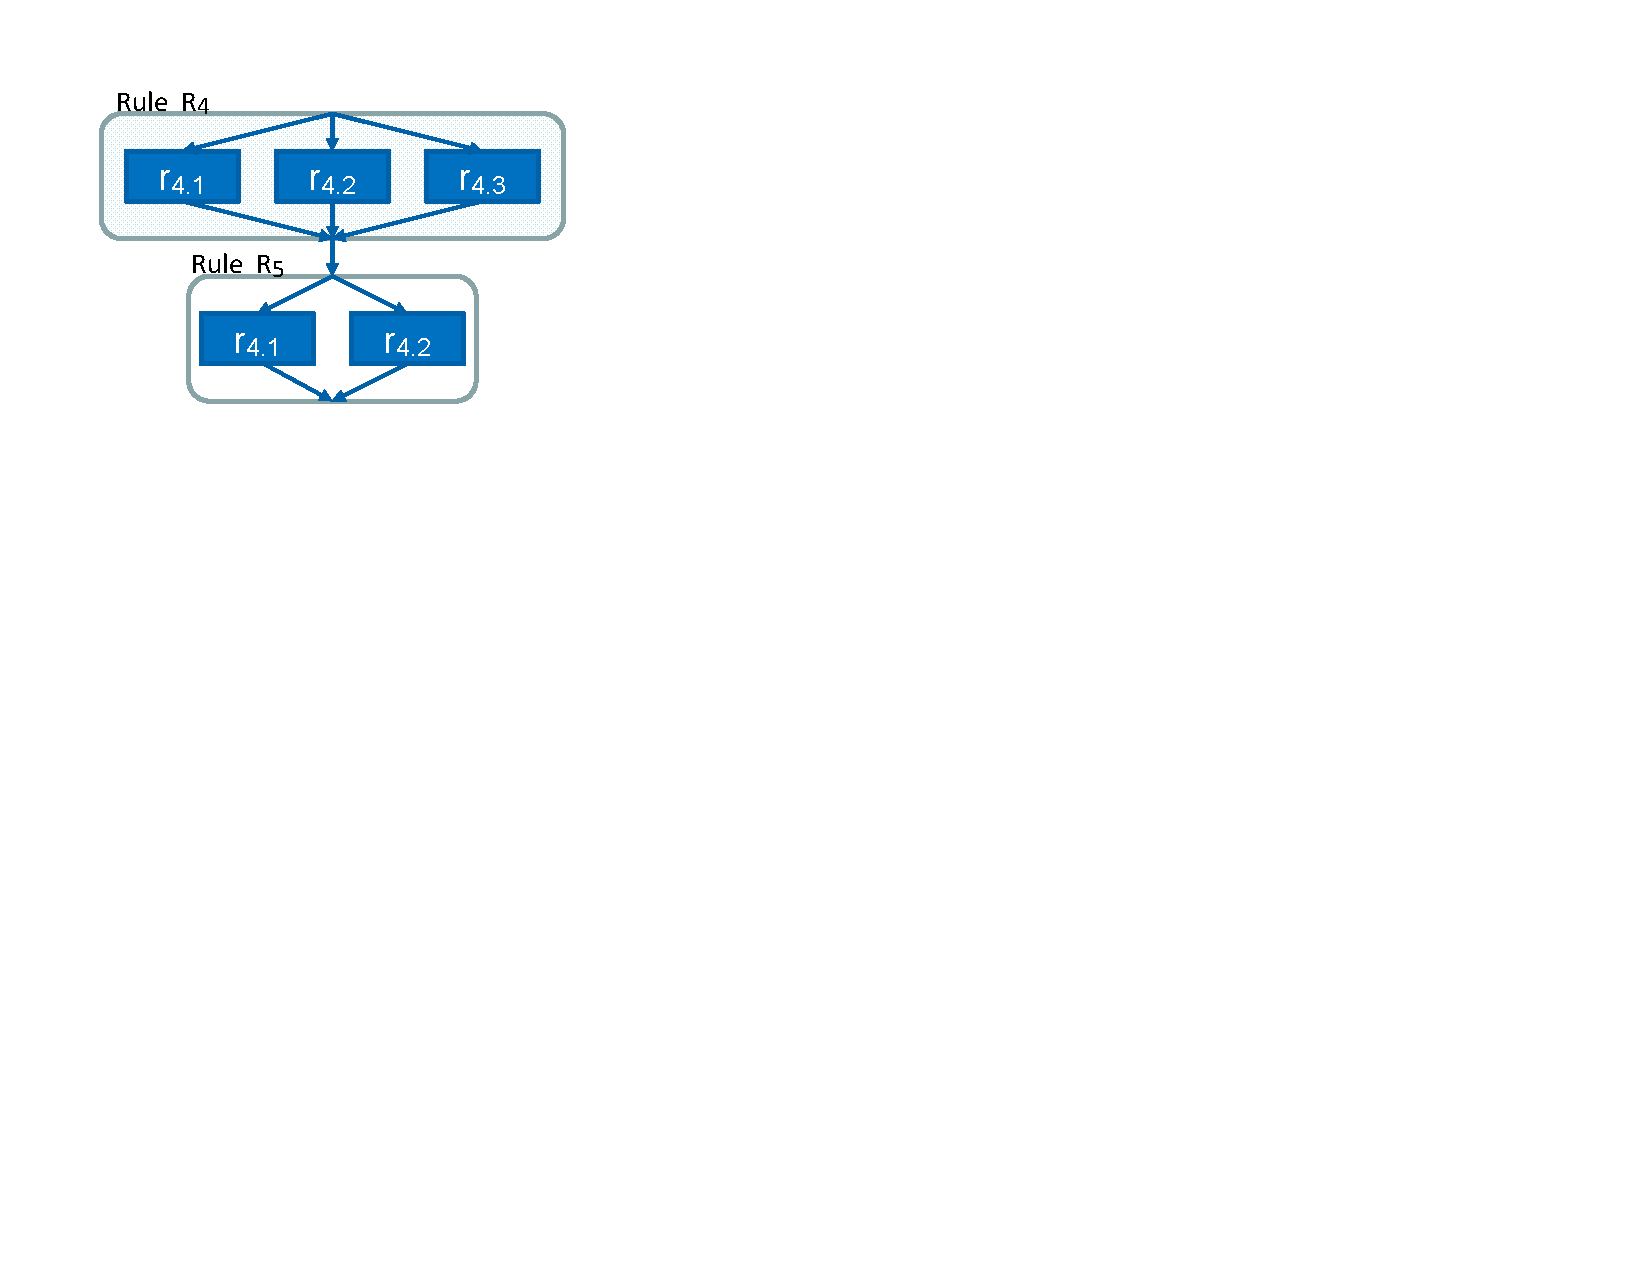
\includegraphics[trim=47 390 520 47,clip,width=.5\columnwidth]{figs/cfg-example.pdf}
\vspace*{-20pt}
\caption{Operation flow graph for \subject{GenerateInvoice}.}
\label{fig:cfg}
\end{figure}

\vskip -7pt
\paragraph*{Operation Flow Graph} To identify combinations of rule parts (within
an operation) that create different object states of entities, we model an
operation as a flow graph. The \textit{operation flow graph} for an operation is
a directed graph consisting of rule subgraphs---one per rule of the
operation---and edges representing flow among the rule subgraphs. A \textit{rule
  subgraph} consists of a unique entry point, a unique exit point, and nodes
that represent rule parts; the subgraph contains an edge from the entry point to
each node and an edge from each node to the exit point.  Figure~\ref{fig:cfg}
illustrates the operation flow graph for \subject{GenerateInvoice} with two
rules, $R_4$ and $R_5$, which have three and two rule parts, respectively.

Because preconditions of all rule parts in a rule are disjoint (Property~1,
Section~\ref{sec:model}), control flow through a rule covers exactly one rule
part.  The rule subgraph captures this aspect by representing each rule as a
choice among its rule parts. Moreover, because there are no data dependences
between rules of an operation (Property~4, Section~\ref{sec:model}), the rule
subgraphs can be composed in any order in the operation flow graph (\ie all
orderings are equivalent).

\subsubsection{Operation Sequences}

\vskip -10pt
\paragraph*{Abstract Sequence} An \textit{abstract sequence} is a sequence of
operations describing flow of objects among the operations such that all
variables that represent instances of entities are defined and other variables
(of enumerated and primitive types) need not be defined. An example abstract
sequence for \subject{GenerateInvoice} is:

\vspace*{-4pt}
{\scriptsize
\begin{alltt}
 CreateCustomer(State st, BalanceType bt, out: Customer cust);
 CreateOrder(Customer cust, out: Order ord);	
 CreateItem(int price, out: Item item);
 AddItemToOrder(Order ord, Item item, out: Order ord1);
 GenerateInvoice(Order ord1, out: Invoice inv);  
\end{alltt}
}
\vspace*{-5pt}

In the notation, variables that are created or modified by an operation are
represented using the keyword \subject{out}. As shown, all variables are
instances of entities are initialized within the sequence.

\vskip -7pt
\paragraph*{Concrete Sequence} A \textit{concrete sequence} constrains an
abstract sequence with selected rule parts for each operation. For an operation,
there can be multiple rule parts selected from different rules of the
operation. Our technique uses concrete sequences to generate test data by
leveraging a constraint solver: it builds a logical formula from concrete
sequences using preconditions and postconditions of all rule parts, and uses
constraint solver to check whether the formula is satisfiable. An example
concrete sequence for the preceding abstract sequence is:

\vspace*{-4pt}
{\scriptsize
\begin{alltt}
 CreateCustomer(State st, BalanceType bt, out: Customer cust) [\(r\sb{1.1}\)];
 CreateOrder(Customer cust, out: Order ord) [\(r\sb{3.1}\)];	
 CreateItem(int price, out: Item item) [\(r\sb{2.1}\)];
 AddItemToOrder(Order ord, Item item, out: Order ord1) [\(r\sb{7.1}\)];
 GenerateInvoice(Order ord1, out: Invoice inv) [\(r\sb{4.1}\)];  
\end{alltt}
}
\vspace*{-5pt}

\subsection{The Algorithm}
\label{sec:technique}

The test-generation algorithm (shown as Algorithm~\ref{alg:guidedsearch}) takes
as inputs an operation ${\cal O}$ and a rule part $r$, and generates a concrete
sequence $seq$ that cover $r$. To illustrate the algorithm, we consider the
operation \subject{GenerateInvoice} and rule part $r_{4.2}$. For brevity, we
omit details such as exiting the main loop (lines~6--15) when the user-defined
threshold of maximum number of sequences to be explored is reached.

\begin{algorithm}[t]
\small
\SetAlgoVlined
\KwIn{Operation ${\cal O}$, Rule part $r$}
\KwOut{Concrete sequence $seq$ or $null$}
\BlankLine

\nl Let $q$ represents a queue of concrete sequences\;
\nl Generate all initialization sequences $iseqs$ for ${\cal O}$\;
\nl \ForEach {sequence $iseq \in iseqs$}
{
		\nl Generate all concrete sequences $cseqs$ for $iseq$\;
		\nl Add $cseqs$ to queue $q$\;
} 

\nl \While { q not empty }
{
		\nl Dequeue sequence $cseq$ from $q$\;
		\nl Check whether $cseq$ is satisfiable\;
		\nl \If {satisfiable}
		{
				\Return $cseq$\;
		}
		
		\nl Extract unsatisfiable core $ucore$ of $cseq$\;
		
		\nl \If {$cseq$ not helping to make progress}
		{
				{\bf continue}\;
		}
		
		\nl Identify operations $ops$ that help satisfy $ucore$\;		
		\nl \ForEach {operation $op \in ops$}
		{
			\nl Generate new sequences $nseqs$ by adding $op$ to $cseq$\;
			\nl Add all $nseqs$ to queue $q$\;
		}
}

\Return $null$\;
		
\caption{\label{alg:guidedsearch} The algorithm for
  generating a concrete sequence that covers a given rule part.}
\end{algorithm}

\vskip -7pt
\paragraph*{Generate Initialization Sequences (Lines 2--5)} The algorithm first
generates, using the dependence graph, all possible initialization sequences
that produce input entities of ${\cal O}$. An initialization sequence is an
abstract sequence, with the restriction that it includes only those operations
that create entities. To create the initialization sequences, the algorithm
identifies input entities $I = \{i_1, i_2, \ldots, i_m\}$ of ${\cal O}$ through
\textit{reads} edges in the dependence graph. For each $i_k$, it identifies the
operations $OP_k = \{{\cal O}^k_1, {\cal O}^k_2, \ldots, {\cal O}^k_n\}$ that
create $i_k$ through \textit{creates} edges in the graph.
%% (Multiple operations can create an entity.)
Then, it computes combinations of all operations across each set corresponding
to $i_k$ to generate initialization sequences. Therefore, for $m$ input entities
and $n$ operations that create each entity, the algorithm generates $n^m$
initialization sequences. Note that the order of operations among the sequences
does not matter because the operations create different entities.  In theory,
the number of initialization sequences could be high; however, in our empirical
evaluation, we found that the number of operations that create entities is often
quite low, resulting in a few initialization sequences only.

The algorithm checks whether any operation in $OP_i$ further requires additional
entities, and repeats this process until no new input entities are required in
all initialization sequences.  For our illustrative example, the initialization
sequence for the operation \subject{GenerateInvoice} is:

\vspace*{-4pt}
{\scriptsize
\begin{alltt}
 CreateCustomer(State st, BalanceType bt, out Customer cust);  
 CreateOrder(Customer cust, out: Order ord);
 GenerateInvoice(Order ord, out: Invoice inv);  
\end{alltt}
}
\vspace*{-5pt}

Next, for each initialization sequence, the algorithm generates concrete
sequences by computing all possible combinations of rule parts among operations
in the sequence. To do this, it joins the operation flow graphs for the
operations and enumerates all paths in the composed flow graph. The concrete
sequences generate different object states for input entities of~${\cal O}$. For
our running example, there is only one concrete sequence because each operation
in the initialization sequence has only one rule part:

\vspace*{-4pt}
{\scriptsize
\begin{alltt}
 CreateCustomer(State st, BalanceType bt, out: Customer cust) [\(r\sb{1.1}\)];
 CreateOrder(Customer cust, out: Order ord) [\(r\sb{3.1}\)];	
 GenerateInvoice(Order ord, out: Invoice inv) [\(r\sb{4.2}\)];  
\end{alltt}
}
\vspace*{-5pt}

\vskip -7pt
\paragraph*{Check Satisfiability (Line 8)} Next, the algorithm checks whe\-ther 
the concrete sequences in the queue are satisfiable. A concrete sequence is
satisfiable if it generates desired object states for all input entities of
${\cal O}$ that cover the precondition of the target rule part. To achieve this,
the algorithm constructs a logical formula composed of constraints in
preconditions and postconditions in each rule part of the sequence and leverages
a constraint solver to check whether the composed formula is satisfiable.

For illustration, consider the sequence of operations with selected rule parts
as $({\cal O}_1 [r_{1.1}], {\cal O}_2 [r_{2.1}], \ldots, {\cal O}_n [r_{n.1}],
{\cal O} [r])$.  The algorithm starts with the precondition of $r$ (referred to
as $target$) in operation ${\cal O}$.  It generates binding constraints that
substitute the entities consumed by ${\cal O}$ with the entities created or
modified by the predecessor operation ${\cal O}_n$. The binding constraints bind
the identifiers in the postcondition of $r_{n.1}$ to the identifiers of the same
type in the precondition of $r$. Because the solver has no notion of objects,
the binding constraints ensure that referenced object attributes are
appropriately bound as well.

The binding constraints are generated as follows. Let $v$ be an identifier of
type $\tau$ occurring in the creates or modifies clause of a predecessor (\eg
${\cal O}_n$) and let $w$ be an identifier of the same type occurring in the
input clause of the successor (\eg ${\cal O}$). If $\tau$ is an enumerated or
primitive type, the only binding constraint needed is $w = v$. However, if
$\tau$ is an object type, we must bind all attributes as well, yielding the
following constraint:

$b_n$: $w = v \wedge w.f_1 = v.f_1 \wedge \ldots \wedge w.f_n = v.f_n$ 

Here, $f_1, \ldots , f_n$ are attributes of $\tau$. To generate the final
binding constraint, this process is applied recursively on each attribute of
object type. Using binding constraints, the algorithm generates the formula as
$p_{n.1} \wedge q_{n.1} \wedge b_n \wedge p$, where $p_{n.1}$ and $q_{n.1}$ are
the precondition and postcondition of $r_{n.1}$. The algorithm checks whether
the composed formula is satisfiable.  If it is, this formula becomes the next
$target$ and ${\cal O}_{n-1}$ the predecessor operation, and the algorithm
repeats the same process with other operations in the sequence.  Once it has
processed all operations in the sequence and the formula is satisfiable, it
extracts values for variables of primitive and enumerated types from the
constraint solution to generate test data.

For our running example, the solver returns that the composed formula as
unsatisfiable. The reason is that $r_{3.1}$ of \subject{CreateOrder} assigns
zero to attribute \subject{total} of \subject{Order}, whereas the precondition
in rule part $r_{4.2}$ of \subject{GenerateInvoice} requires the value of
\subject{total} to be greater than zero.

\vskip -7pt
\paragraph*{Extract Unsatisfiable Core (Line 10)} If the composed formula is
unsatisfiable, the algorithm extracts the unsatisfiable core, \subject{ucore},
of the formula. The unsatisfiable core is a subset of the formula that preserves
the unsatisfiability but is simplified compared to the original formula.
\subject{ucore} guides the algorithm toward other operations that modify
attributes of entities to produce the goal object
states. (Section~\ref{sec:impl} presents the implementation details of how we
extract \subject{ucore} from a formula.)

For our example, the algorithm extracts \subject{ucore} as \subject{ord.total =
  0 $\wedge$ ord.total > 0}, composed of constraints from rule parts $r_{3.1}$
and $r_{4.2}$. For ease of explanation, we discuss line~11 after explaining the
rest of the algorithm.

%If the unsatisfiable core is already seen for this sequence, our algorithm
%ignores the sequence. The reason is that the candidate operation that is suggested
%earlier did not help make any additional progress by resulting in the same unsatisfiable core.
%TODO: Refer to Tao's DSN paper for fitness functions.

\vskip -7pt
\paragraph*{Identify Candidate Operations (Line 12)}
%% Since our algorithm checks satisfiability for each operation in the sequence
%% beginning from the last operation, when we extract unsatisfiable core, it
%% contains constraints from the formula that was composed so far and also the
%% constraints from the last analyzed operation.
Before searching for other candidate operations, the algorithm discards
constraints from \subject{ucore} that are contributed by the last analyzed
operation (as these constraints cause the unsatisfiability of $target$).  We use
the notation \subject{ucore-} to represent the remaining constraints in the
extracted unsatisfied core. The intuition behind computing \subject{ucore-} is
to identify candidate operations that are compatible with \subject{ucore-} so
that the composed formula can be satisfiable.  The algorithm first extracts
entities and their attributes involved in \subject{ucore-}. Next, it identifies
candidate operations that modify those entities.  For each such candidate
operation, it identifies rule parts that modify the desired attributes and also
whose postconditions are compatible with \subject{ucore-}, \ie{} $q \wedge b
\wedge \subject{ucore-}$ is satisfiable, where $q$ is the postcondition of the
selected rule part in the candidate operation and $b$ represents binding
constraints.  This additional satisfiability check helps discard candidate
operations that do modify the desired attributes but still cannot help in
identifying a covering sequence for $r$; this can significantly reduce the
search space of candidate sequences.

For our illustrative example, our algorithm computes \subject{ucore-} as
\subject{ord.total > 0}, and identifies the entity as \subject{Order} and the
desired attribute to be modified as \subject{total}. It analyzes all operations
that create or modify \subject{Order}, and identifies two candidate operations
as \subject{CreateOrder} and \subject{AddItemToOrder} and rule parts as
$r_{3.1}$ and $r_{7.1}$, respectively, in those operations.  It discards
\subject{CreateOrder} because $q_{3.1} \wedge \subject{ucore-}$ is not
satisfiable, but selects \subject{AddItemToOrder} because $q_{7.1} \wedge
\subject{ucore-}$ is satisfiable.

%TODO: write about searching operations that modify parent entites as well.

\vskip -7pt
\paragraph*{Generate Alternate Sequences (Lines 13--15)} After a candidate
operation (along with relevant rule parts) is identified, the algorithm checks
whether any additional input entities that are not yet available in the current
sequence $cseq$ are required by that operation.  If so, it identifies the
additional operations that create those entities. Then, using the dependence
graph, it identifies all positions in $cseq$ where the candidate operation
(along with the additional operations) can be inserted. Note that there can be
multiple positions that satisfy dependencies for inserting the candidate
operation, and the resulting sequences can produce different object states for
the input entities of ${\cal O}$.  Therefore, the algorithm can generate
multiple sequences while inserting candidate operation into $cseq$. Finally, the
algorithm adds all newly generated sequences to the queue to further analyze
those sequences.

For our running example, because \subject{AddItemToOrder} requires an additional
entity \subject{Item} that is not available in the sequence, the algorithm adds
operation \subject{CreateItem} as well to the newly generated sequence. After
creating the new concrete sequence, it checks satisifiability of the new
sequence, where it further detects the unsatisfiable core as
\subject{cust.crLimit = 0 $\wedge$ cust.crLimit > 0}.  It then repeats the loop
(lines~6--15), and identifies the final concrete sequence that covers $r_{4.2}$
as follows:

\vspace*{-4pt}
{\scriptsize
\begin{alltt}
 CreateCustomer(State st, BalanceType bt, out: Customer cust) [\(r\sb{1.1}\)];
 AddCreditLimit(Customer cust, int crLimit, out: Customer cust1) [\(r\sb{6.1}\)];
 CreateOrder(Customer cust, out: Order ord) [\(r\sb{3.1}\)];
 CreateItem(int price, out: Item item) [\(r\sb{2.1}\)];
 AddItemToOrder(Order ord, Item item, out: Order ord1) [\(r\sb{7.1}\)];
 GenerateInvoice(Order ord1, out: Invoice inv) [\(r\sb{4.2}\)];  
\end{alltt}
}
\vspace*{-5pt}

\vskip -7pt
\paragraph*{Check Progress (Line 11)} We next explain the significance of the
conditional check in line~11, which ensures that the algorithm makes progress
over iterations.  While identifying candidate operations, the algorithm discards
those operations that do not help cover the target rule part (line~12). However,
in a few cases, even the selected operations may not help make progress and need
to be discarded to make the exploration efficient. To identify such cases, the
algorithm checks the following two aspects for each $cseq$.

First, if the extracted unsatisfiable core \subject{ucore} was already seen in
previous iterations related to $cseq$, the algorithm discards $cseq$. The reason
is that the candidate operation that was added to $cseq$ in the previous
iteration did not help satisfy the previous \subject{ucore}, resulting in the
same \subject{ucore} in the next iteration as well.

Second, when \subject{ucore} includes integer variables, our algorithm uses a
fitness function to measure whether $cseq$ helps get closer to cover the rule
part $r$ or not. The first check is sufficient for boolean variables or
variables of enumerated types but is insufficient to deal with the integer
variables.

To illustrate the issue, suppose that our model includes another operation,
\subject{RemoveItemFromOrder}, that removes a selected item and decreases the
value of attribute \subject{total} of \subject{Order}. While exploring candidate
operations, our algorithm identifies \subject{AddItemToOrder} and
\subject{RemoveItemFromOrder} because both operations modify
\subject{total}. However, \subject{RemoveItemFromOrder} does not help cover
$r_{4.2}$ as it actually decreases the value of \subject{total}. To handle such
cases, the algorithm uses a fitness function, originally proposed in
Fitnex~\cite{xie09:fitness}, to measure whether $cseq$ gets closer to covering
the target rule part. The idea is to compute a fitness value from
\subject{ucore} and if this value is better than the fitness value computed
during the previous iteration, $cseq$ is processed further; otherwise, it is
discarded.

\section{Empirical Evaluation}
\label{sec:eval}

We implemented our technique in a prototype tool called \tool{} (BUSiness
TEsting Rules), and conducted two empirical studies using two open-source
applications and one proprietary enterprise application. In the first study, we
compared the effectiveness of \tool{} in covering business rules with a related
technique that systematically explores the search space without any guidance. In
the second study, we investigated the efficiency of both the techniques. %% After
%% describing the experimental setup, we present results of the two studies.

\subsection{Experimental Setup}
\label{sec:impl}
\vspace*{-3pt}
\paragraph*{Implementation} Our implementation \tool{}  uses \choco{} constraint
solver~\cite{Choco} for checking the satisfiability of sequences. Since \choco{}
does not provide functionality for extracting unsatisfied core, we use a
heuristic-based implementation to extract the core. While checking whether a
concrete sequence is satisfiable, \tool{} starts with the last operation of the
sequence and performs backward analysis by handling each operation and their
rule parts. Therefore, when a composed formula is unsatisfiable, it can be
caused only by a constraint in the most recently analyzed rule part. Next, it
uses the variables involved in that constraint to extract the complete
unsatisfied core. Note that \tool{} may not extract the minimal unsatisfied
core; however, the extracted core is sufficient to suggest candidate
operations. We leave improvements in the implementation to future work, for
example, by exploring advanced algorithms for extracting unsatisfied
core~\cite{Liffiton:2008:ACM} and also leverage other constraint
solvers~\cite{DeMoura:2008}. Another optimization could include caching and
reusing constraints (\eg as discussed in the Green approach~\cite{VisserGD12}).

\begin{table}[t]
\caption{Subjects used in our empirical studies.}
\vskip -5pt
\centering
{\scriptsize
\tabcolsep=3pt
\begin{tabular}{|l|l|r|r|r|r|}
\hline
\multicolumn{1}{|c|}{Subject} & \multicolumn{1}{|c|}{URL} & \multicolumn{1}{|c|}{Entities} & \multicolumn{1}{|c|}{Operations} & \multicolumn{1}{|c|}{Rules} & \multicolumn{1}{|c|}{Rule parts} \\
\hline \hline
Cebu-pacific & www.cebupacificair.com 		& 8  & 10 & 15	 & 31 \\
jBilling 		 & www.jbilling.com 					& 10 & 10 & 14 	 & 26 \\
App 				 & \multicolumn{1}{|c|}{---}	& 12 & 13 & 13   & 20 \\
\hline \hline
\textbf{Total} & 													& 	 & 33 & 42   & 77 \\
\hline
\end{tabular}
}
\label{tab:subjects}
\end{table}


To compare \tool{} with an unguided search over the space of candidate
sequences, we implemented another tool, called \exhaust{}, which is similar to
\tool{}, but without the optimizations presented in
Section~\ref{sec:optimization}. As an unguided technique, \exhaust{} lets us
evaluate the effectiveness of leveraging unsatisfied core to guide the search
for covering sequences.

%that systematically explores sequences without guidance via
%unsatisfied core. Similar to \tool{}, \exhaust{} uses a queue $q$ to store
%candidate sequences. Given an operation ${\cal O}$ and a target rule part $r$,
%\exhaust{} first creates a sequence $seq$ with ${\cal O}\ [r]$ and adds $seq$ to
%$q$. For each $seq$, \exhaust{} associates a list of input entities, referred to
%as \subject{ilist}.  Initially, \subject{ilist} contains the input entities of
%${\cal O}$ only.  Next, \exhaust{} dequeues a sequence $qseq$ from $q$, removes
%an entity from \subject{ilist}, and identifies all operations \{${\cal O}_1,
%{\cal O}_2, \ldots, {\cal O}_n$\} that create or modify that entity. \exhaust{}
%creates new sequences by adding each ${\cal O}_i$ to $qseq$. Also, if an ${\cal
%  O}_i$ requires additional input entities, it adds those entities to the
%\subject{ilist} for the newly created sequence. Next, it adds the new sequences
%to $q$ and repeats the process. When \exhaust{} encounters a concrete sequence,
%\ie{} a sequence whose \subject{ilist} is empty, it uses \choco{} to check
%whether the sequence is satisfiable: if it is, \exhaust{} returns the sequence
%and terminates; otherwise, it continues analyzing other sequences in
%$q$. \exhaust{} repeats this process until it finds a satisfiable sequence or
%reaches the user-defined upper bound on the number of sequences to be explored. 

\paragraph*{Subjects and Rules} We used two open-source applications and a proprietary enterprise application,
listed in Table~\ref{tab:subjects}, as the experimental subjects. Due to
confidentiality reasons, we refer to the proprietary application as
\subject{App}. \subject{Cebu-pacific} is an airlines application,
\subject{jBilling} is an enterprise billing application, and \subject{App} is a
telecom application. Column~2 shows the URLs of the first two subjects.
Columns~3--6 show additional details, such as the number of entities,
operations, and rules. For each subject, we identified a module that is likely
to have large number of interesting rules with respect to the sequences and test
data required for coverage, and modeled those modules using our tool. In
particular, we used the \textit{ticket cancellation} and \textit{generate
  invoice} modules for \subject{Cebu-pacific} and \subject{jBilling},
respectively. In total, we modeled $33$ operations with $42$ rules and $77$ rule
parts.\footnote{The complete dataset including models and the
  generated test sequences is available at \url{http://tinyurl.com/k4b4j8x}
  (also available on request from the authors).} For each subject, we spent
approximately~10 hours to model the operations and rules. We also found that
our rule editor and property checking helped create correct rule set.

\paragraph*{Method} We applied \tool{} and \exhaust{} on the models created for each subject and
generated test sequences. For each rule part, we let each tool explore up to a
maximum of $100$ concrete sequences. Next, we inspected the generated sequences
to ensure that they cover the targeted rule parts. To evaluate the efficiency of
the tools, we measured the number of sequences explored and the lengths of
sequences produced by each tool.  All experiments were conducted on an Intel
Core 2 Duo CPU machine with 2.53 GHz and 8GB RAM. Next, we present the results
of the studies.

\subsection{Coverage of Business Rules}

\begin{figure}[t]
\centering
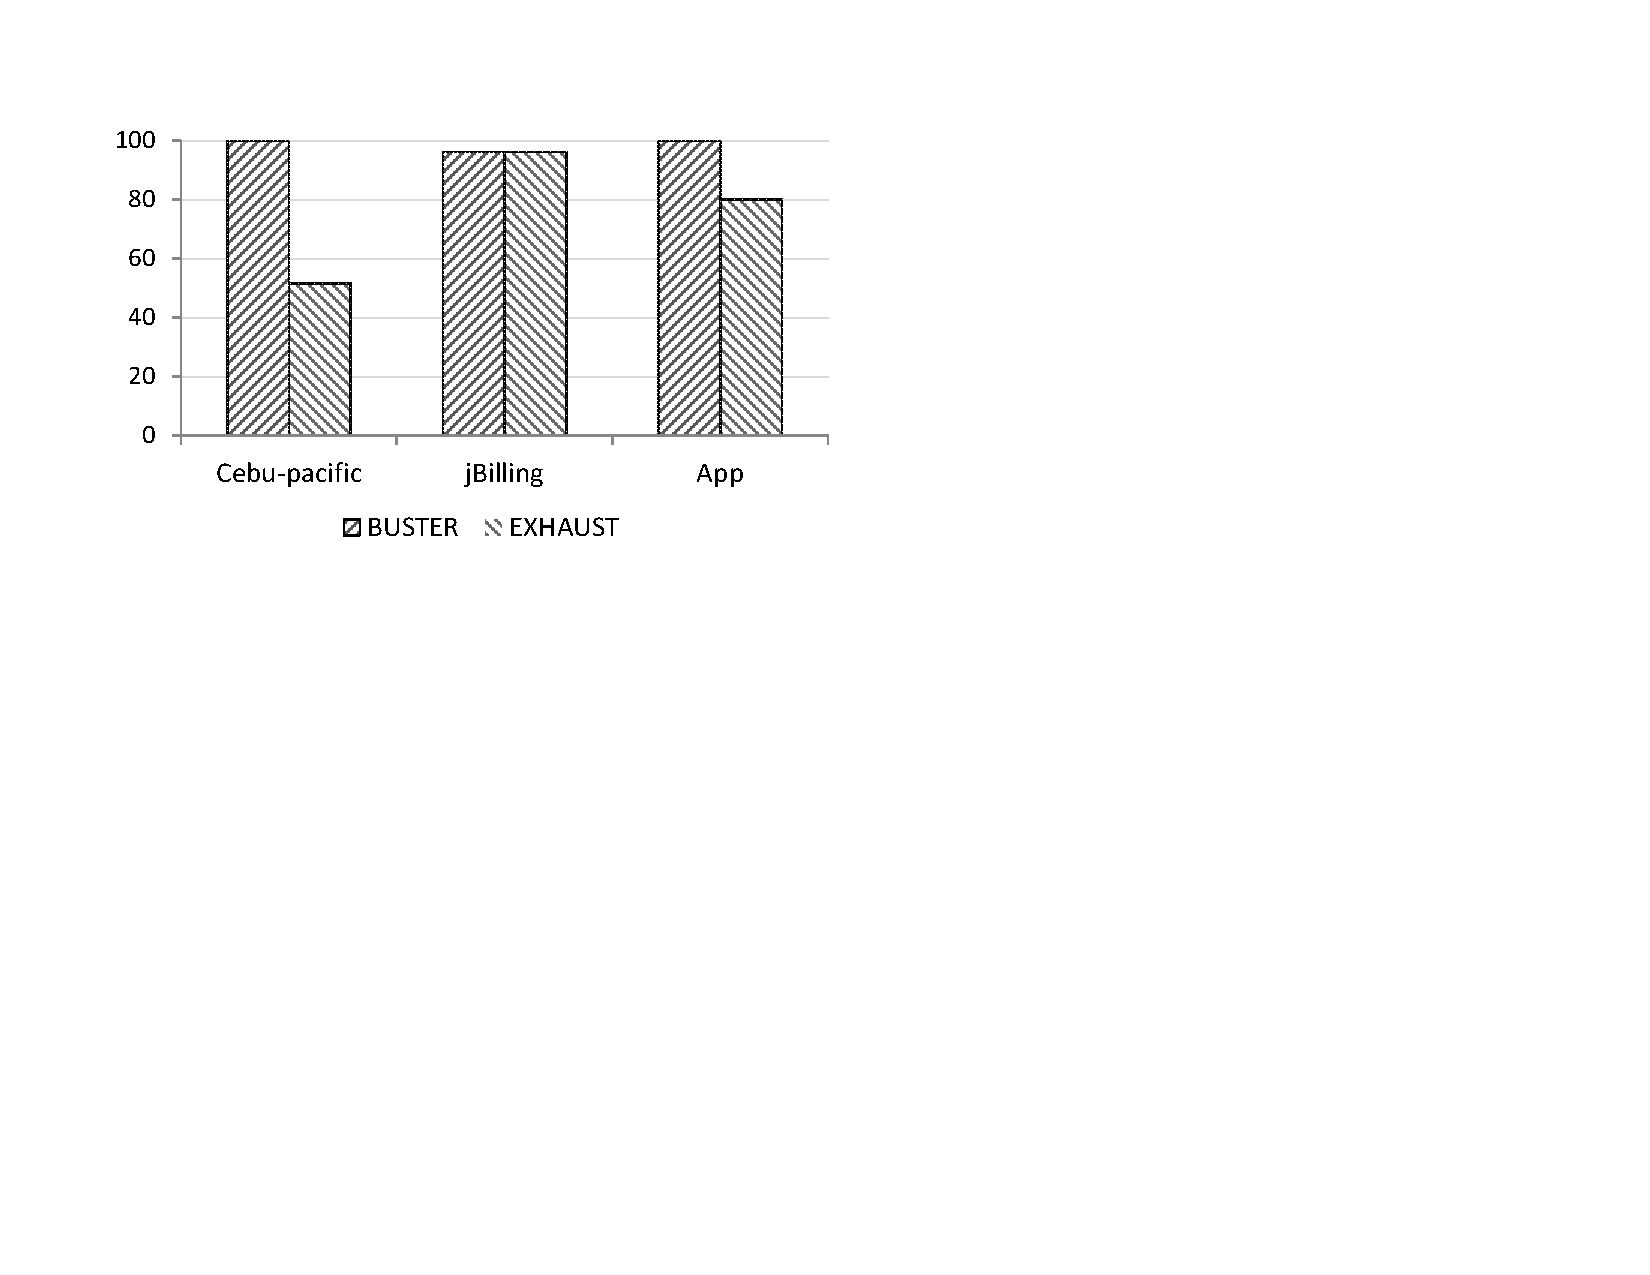
\includegraphics[width=0.65\columnwidth, clip, trim = 18mm 120mm 140mm
  18mm]{figs/Study-1.pdf}
\vspace*{-10pt}
\caption{Effectiveness of the two techniques in covering business rules.}
\label{fig:effectiveness}
\end{figure}

Figure~\ref{fig:effectiveness} presents the results for all three subjects: it
shows the percentages of rule parts covered by each tool. For example, for
\subject{Cebu-pacific}, \tool{} generated covering sequences for all $31$ rule
parts, whereas \exhaust{} was able to generate sequences only for $16$ rule
parts. Overall, the results show that \tool{} covered $99$\% of the rule parts,
whereas \exhaust{} could cover only $74$\% of the rule parts.

We further analyzed the cases where the tools could not cover the targeted rule
parts. We found that, in general, \exhaust{} performs poorly if there are many
operations that create or modify the required input entities. This is expected
because it results in a large search space of candidate operation sequences,
which \tool{} is able to navigate effectively in a goal-directed manner (guided
by the unsatisfied core), whereas \exhaust{} has to try the candidate sequences
in a blind manner. Thus, \exhaust{} performed well on \subject{jBilling}, in
which each entity is created or modified by only a few operations. But, for
\subject{Cebu-pacific}, where some entities are modified by many operations,
\exhaust{} was much less effective. In such cases, a directed search guided by
unsatisfied core, is necessary---and can be highly effective---for attaining
high rule coverage.

For \subject{jBilling}, both \tool{} and \exhaust{} could not cover one rule
part because of an issue with \choco{} solver: \choco{} terminated with an
out-of-memory error while solving the composed formula for that rule part.

%% While analyzing our results, we identified that the rule parts that were not
%% covered by \exhaust{} require complex sequences. In particular, \exhaust{} could
%% handle subjects such as \subject{jBilling}, where there are only a few
%% operations that create or modify each entity. On the other hand, it could not
%% handle subjects such as \subject{Cebu-pacific}, where there are several
%% operations that modify the same entity. Both \tool{} and \exhaust{} could not
%% cover one rule part in \subject{jBilling} due to an issue with \choco{}
%% solver. \choco{} produced out of memory error while solving the composed formula
%% for that rule part.

Next, we illustrate a complex sequence generated by \tool{} for a rule part in
\subject{Cebu-pacific}. This rule part pertains to fare refunds because of
flight cancellation due to a delay of more than two
hours. \subject{Cebu-pacific} allows a ticket to be booked as multiple sectors,
where each sector represents part of the journey from one city to another
city. The airlines has a refund policy that if the flight corresponding to any
sector gets canceled due to a delay of more than two hours, passengers can get a
refund so as to make alternative travel arrangements. To cover this rule part
that belongs to operation \subject{Refund}, a specific instance of
\subject{Ticket} entity is required. First, the ticket should include at least
one sector and the passenger should have sufficient funds to add a sector to the
ticket. Next, the flight corresponding to that sector should be delayed by more
than two hours and, consequently, canceled. \tool{} successfully generated the
following covering sequence and test data, whereas \exhaust{} failed to generate
a covering sequence.

{\scriptsize
\begin{alltt}
 int fund = 200, passenger = 1, delay = 3, sectorid = 1;
 Fund fund = CreateFund(fund, passenger);
 Ticket ticket = CreateTicket(passenger);
 int flight = 901, price = 100, departure = 10; 
 Sector sector = MakeSector(flight, price, departure);
 AddSector(ticket, sector, fund, out Ticket ticket1, out Fund f1); 
 Ticket ticket2 = DelayFlight(ticket1, sectorid, delay);
 Ticket ticket3 = PartialCancellation(ticket2, sectorid);
 Refund(ticket3, sectorid, f1, out Ticket ticket4, out Fund f2);
\end{alltt}
}

Overall, our results illustrate the promise of our technique in effectively
generating complex sequences for covering business rules.

\begin{table}[t]
\caption{Efficiency of \tool{} and \exhaust{}.}
\centering
{\scriptsize
\tabcolsep=3pt
\begin{tabular}{|l|r|r|r|r|r|r|r|r|r|r|}
\hline
& \multicolumn{4}{|c|}{Sequence Length} & \multicolumn{4}{|c|}{\# of Sequences Explored} & \multicolumn{2}{|c|}{Time (sec)} \\
\cline{2-11}
& \multicolumn{2}{|c|}{\tool{}} & \multicolumn{2}{|c|}{\exhaust{}} &
\multicolumn{2}{|c|}{\tool{}} & \multicolumn{2}{|c|}{\exhaust{}} &
\multicolumn{1}{|c|}{\tool{}} & \multicolumn{1}{|c|}{\exhaust{}} \\
\cline{2-9}
\multicolumn{1}{|c|}{Subject} & \multicolumn{1}{|c|}{Max} & \multicolumn{1}{|c|}{Avg} & \multicolumn{1}{|c|}{Max} & \multicolumn{1}{|c|}{Avg} & \multicolumn{1}{|c|}{Max} & \multicolumn{1}{|c|}{Avg} & \multicolumn{1}{|c|}{Max} & \multicolumn{1}{|c|}{Avg} & &  \\
\hline \hline
Cebu-pacific 	 &  7		& 5 &  9 &  5	 &  27 &  4	&  100 & 73 & 31 & 64 \\
jBilling		 	 &  6		& 3 &  6 &  3	 &  48 &  2	&  39  &  2 & 20 & 17 \\
App					 	 &  9		& 6 & 10 &  6	 &  51 &  5	& 100  & 46 &  4 & 12 \\
\hline
\end{tabular}
}
\label{tab:stats}
\end{table}

\subsection{Efficiency}

Table~\ref{tab:stats} presents data about the lengths of sequences and the
number of sequences generated by \tool{} and \exhaust{}. Columns~2--5 show the
maximum and average lengths of sequences generated for all rule parts, whereas
Columns~6--9 show the number of sequences explored by each tool for all rule
parts. Finally, Columns~10--11 show the time taken (in seconds) by each tool.

The results show that, in some cases, \tool{} generated relatively shorter
sequences compared to \exhaust{}. More significantly, \tool{} explored much
fewer sequences than \exhaust{}. For example, for \subject{Cebu-pacific},
\tool{} explored on average only $4$ sequences (maximum of $27$), whereas
\exhaust{} explored on average $73$ sequences for each rule part (and also hit
the upper bound of $100$ sequences). In none of the cases, \tool{} terminated by
reaching the upper bound. Overall, these results indicate that guided search via
unsatisfied core can make \tool{} highly efficient compared to \exhaust{}. 
The results show that the time taken by each tool correlates with the
number of sequences explored.

%\subsection{Discussion}
%
%These results illustrate the promise of our technique. But, further
%experimentation with more varied subjects and business rules are
%required to confirm the generality of, and increase our confidence in,
%these observations.
%
%This work partially fulfills our vision of making the testing of enterprise
%applications more tool-based. Our longer-term goal is to generate executable
%test cases that drive the application via its GUI---as illustrated by the flow
%depicted in Figure~\ref{fig:jbilling-flow}---to test the application's
%conformance to business rules. Toward that goal, we plan to leverage our
%previous work~\cite{Thummalapenta:2013}, in which we developed a tool, \wateg{},
%that performs directed crawling of a web application to generate executable GUI
%test cases. \wateg{} also takes as input a specification of rules, but those
%rules are expressed in terms of the GUI elements (\eg links, buttons, and text
%boxes) of an application, and pertain to access-control properties, navigational
%properties, and so on.  A natural integration between this work and
%\wateg{}-style crawling technology would be to extend our rule-modeling language
%to accommodate \textit{flow specifications} for operations, which (along with
%the test data) could be provided as input to \wateg{} to generate executable
%rule-covering tests.

% !TEX root = paper.tex
\section{Related work}

At first blush, this problem seems to be reminiscent of the problem of
generating tests for programs written as control-flow graphs, with the
goal of exercising each acyclic path in the program, if possible.
There have been a number of techniques in the literature for test
generation. Mostly notably, techniques such as \textit{concolic}
testing attempt to identify a series of test data that would force
program execution thorough different paths~\cite{dart, concolic}.  Other
approaches are based on model checking, with the goal of creating test
inputs to reach specific program states.

However, the problem of test generation from business rules is
different. Business rules do not describe the implementation of a
system: rather they only describe a model and many of the concerns
that arise when dealing with control flow graph derived from real code
are not pertinent.

\subsection{Model based testing}

The set of business rules can viewed as a model of an actual system
that supports them and our approach then becomes a variant of model
based test generation~\cite{utting2012}. Compared to the formalisms commonly used in the
literature our business rule language is more light weight. We do not
require the programmer to specify control flow properties or other
program level details.

Typical modeling languages used by model based testing systems include
UML sequence diagrams~\cite{nayak2009}, modeling specific languages
such as the Systems Modeling Language~\cite{friedenthal2011} and
finite state machine notations such as UML
state charts~\cite{offhut99}. While business rules as presented in this
paper could be expressed in any of these notations it would be
cumbersome and require some degree of non-trivial encoding on part of
the author, making it unattractive to a non-programmer. Our business
rule language is designed so that rules are written in much the same
way as one would write them in prose thereby making it more accessible
to non-programmers.

Sriganesh and Ramanathan~\cite{sriganesh2012} extract business rules
from systems described in the Business Process Model and Notation
language, a graphical notation used to describe business
processes. The rule output is in a format similar to our formalism and
our algorithm could conceivably be applied to generate test sequences
from these rules.

\subsection{AI Planning}

Previous work has applied AI planning to software
testing~\cite{Scheetz99ai,Howe97testcase}. The sequencing of
operations done by our algorithm is similar to the AI planning
problem~\cite{Weld94} where actions with pre- and postconditions are sequenced
by a planner algorithm using either forward or backward chaining. The
algorithms used by AI planners are similiar the naive technique
presented in Section~\ref{sec:eval} which proved insuffecient for our
benchmarks. 

Part of an AI planning problem is the initial state of the program,
including what objects exists and which conditions that can be
assumed. Our technique does not need this: The types of objects that
exist in the system are defined in the model along with operations
that create them. A test sequence will construct any object needed to
cover a given rule part.

Paradkar et al~\cite{conf/icws/ParadkarSWJOSL07}.\ presents a system
for testing web services specified in the semantic markup language
OWL-S. OWL-S represents operations in a manner similar to our language
with pre- and postcondtion. However each operation has only one
associated pre- and postcondition pair making it more akin to a rule
in our language. If one where to translate a model in our business
rule language into OWL-S each rule would have to be turned into a
standalone operation. Such a translation could potentially increase the
size of the search space and lead to spurious sequences being
reported. The focus of the technique presented in the paper is on
conformance testing, that is, testing if a given implementation
conforms to the specification. In our approach the business rules are
the specification and the aim is instead to generates tests that cover
all rules. The paper does not mention the size of the models the
technique was evaluated on or the size of the generated test
sequences.

\subsection{Method Sequence Generation}

When testing object oriented code achieving high coverage of a method
requires driving the reciever object and any objects passed as
arguments into a desired state. The problem of generating a method
sequence to cover a particular method is similar to our problem of
covering a rule part. 



\section{Conclusion}
...


\bibliographystyle{IEEEtran}
{\small
\bibliography{paper}
}
\end{document}
